%**************************************%
%* Generated from MathBook XML source *%
%*    on 2017-05-23T16:41:20-07:00    *%
%*                                    *%
%*   http://mathbook.pugetsound.edu   *%
%*                                    *%
%**************************************%
\documentclass[10pt,]{book}
%% Custom Preamble Entries, early (use latex.preamble.early)
%% Inline math delimiters, \(, \), need to be robust
%% 2016-01-31:  latexrelease.sty  supersedes  fixltx2e.sty
%% If  latexrelease.sty  exists, bugfix is in kernel
%% If not, bugfix is in  fixltx2e.sty
%% See:  https://tug.org/TUGboat/tb36-3/tb114ltnews22.pdf
%% and read "Fewer fragile commands" in distribution's  latexchanges.pdf
\IfFileExists{latexrelease.sty}{}{\usepackage{fixltx2e}}
%% Text height identically 9 inches, text width varies on point size
%% See Bringhurst 2.1.1 on measure for recommendations
%% 75 characters per line (count spaces, punctuation) is target
%% which is the upper limit of Bringhurst's recommendations
%% Load geometry package to allow page margin adjustments
\usepackage{geometry}
\geometry{letterpaper,total={340pt,9.0in}}
%% Custom Page Layout Adjustments (use latex.geometry)
%% This LaTeX file may be compiled with pdflatex, xelatex, or lualatex
%% The following provides engine-specific capabilities
%% Generally, xelatex and lualatex will do better languages other than US English
%% You can pick from the conditional if you will only ever use one engine
\usepackage{ifthen}
\usepackage{ifxetex,ifluatex}
\ifthenelse{\boolean{xetex} \or \boolean{luatex}}{%
%% begin: xelatex and lualatex-specific configuration
%% fontspec package will make Latin Modern (lmodern) the default font
\ifxetex\usepackage{xltxtra}\fi
\usepackage{fontspec}
%% realscripts is the only part of xltxtra relevant to lualatex 
\ifluatex\usepackage{realscripts}\fi
%% 
%% Extensive support for other languages
\usepackage{polyglossia}
\setdefaultlanguage{english}
%% Magyar (Hungarian)
\setotherlanguage{magyar}
%% Spanish
\setotherlanguage{spanish}
%% Vietnamese
\setotherlanguage{vietnamese}
%% end: xelatex and lualatex-specific configuration
}{%
%% begin: pdflatex-specific configuration
%% translate common Unicode to their LaTeX equivalents
%% Also, fontenc with T1 makes CM-Super the default font
%% (\input{ix-utf8enc.dfu} from the "inputenx" package is possible addition (broken?)
\usepackage[T1]{fontenc}
\usepackage[utf8]{inputenc}
%% end: pdflatex-specific configuration
}
%% Monospace font: Inconsolata (zi4)
%% Sponsored by TUG: http://levien.com/type/myfonts/inconsolata.html
%% See package documentation for excellent instructions
%% One caveat, seem to need full file name to locate OTF files
%% Loads the "upquote" package as needed, so we don't have to
%% Upright quotes might come from the  textcomp  package, which we also use
%% We employ the shapely \ell to match Google Font version
%% pdflatex: "varqu" option produces best upright quotes
%% xelatex,lualatex: add StylisticSet 1 for shapely \ell
%% xelatex,lualatex: add StylisticSet 2 for plain zero
%% xelatex,lualatex: we add StylisticSet 3 for upright quotes
%% 
\ifthenelse{\boolean{xetex} \or \boolean{luatex}}{%
%% begin: xelatex and lualatex-specific monospace font
\usepackage{zi4}
\setmonofont[BoldFont=Inconsolatazi4-Bold.otf,StylisticSet={1,3}]{Inconsolatazi4-Regular.otf}
%% end: xelatex and lualatex-specific monospace font
}{%
%% begin: pdflatex-specific monospace font
\usepackage[varqu]{zi4}
%% end: pdflatex-specific monospace font
}
%% Symbols, align environment, bracket-matrix
\usepackage{amsmath}
\usepackage{amssymb}
%% allow page breaks within display mathematics anywhere
%% level 4 is maximally permissive
%% this is exactly the opposite of AMSmath package philosophy
%% there are per-display, and per-equation options to control this
%% split, aligned, gathered, and alignedat are not affected
\allowdisplaybreaks[4]
%% allow more columns to a matrix
%% can make this even bigger by overriding with  latex.preamble.late  processing option
\setcounter{MaxMatrixCols}{30}
%%
%% Color support, xcolor package
%% Always loaded.  Used for:
%% mdframed boxes, add/delete text, author tools
\PassOptionsToPackage{usenames,dvipsnames,svgnames,table}{xcolor}
\usepackage{xcolor}
%%
%% Semantic Macros
%% To preserve meaning in a LaTeX file
%% Only defined here if required in this document
%% Used for inline definitions of terms
\newcommand{\terminology}[1]{\textbf{#1}}
%% Subdivision Numbering, Chapters, Sections, Subsections, etc
%% Subdivision numbers may be turned off at some level ("depth")
%% A section *always* has depth 1, contrary to us counting from the document root
%% The latex default is 3.  If a larger number is present here, then
%% removing this command may make some cross-references ambiguous
%% The precursor variable $numbering-maxlevel is checked for consistency in the common XSL file
\setcounter{secnumdepth}{3}
%% mdframed environments use a tikz frame method
\usepackage{tikz}%% Environments with amsthm package
%% Theorem-like environments in "plain" style, with or without proof
\usepackage{amsthm}
\theoremstyle{plain}
%% Numbering for Theorems, Conjectures, Examples, Figures, etc
%% Controlled by  numbering.theorems.level  processing parameter
%% Always need a theorem environment to set base numbering scheme
%% even if document has no theorems (but has other environments)
\newtheorem{theorem}{Theorem}[chapter]
%% Only variants actually used in document appear here
%% Style is like a theorem, and for statements without proofs
%% Numbering: all theorem-like numbered consecutively
%% i.e. Corollary 4.3 follows Theorem 4.2
%% Remark-like environments, normal text
%% Numbering is in sync with theorems, etc
\theoremstyle{definition}
\newtheorem{remark}[theorem]{Remark}
%% Example-like environments, normal text
%% Numbering is in sync with theorems, etc
\theoremstyle{definition}
\newtheorem{example}[theorem]{Example}
%% Package for breakable highlight boxes
\usepackage[framemethod=tikz]{mdframed}
%% begin: assemblage
%% minimally structured content, high visibility presentation
%% environments (untitled, titled), with style
\newenvironment{assemblage-untitled}{\mdfsetup{%
roundcorner=2ex, backgroundcolor=blue!5,linecolor=blue!75!black,}%
\begin{mdframed}}{\end{mdframed}}
\newenvironment{assemblage}[1]{\mdfsetup{frametitle={\colorbox{blue!20}{\space#1\space}},%
frametitlealignment={\hspace*{1ex}}, frametitleaboveskip=-1.5ex, frametitlebelowskip=0pt,%
roundcorner=2ex, backgroundcolor=blue!5,linecolor=blue!75!black,}%
\begin{mdframed}}{\end{mdframed}}
%% end: assemblage
%% Miscellaneous environments, normal text
%% Numbering for inline exercises and lists is in sync with theorems, etc
\theoremstyle{definition}
\newtheorem{exercise}[theorem]{Exercise}
%% Localize LaTeX supplied names (possibly none)
\renewcommand*{\chaptername}{Chapter}
%% For improved tables
\usepackage{array}
%% Some extra height on each row is desirable, especially with horizontal rules
%% Increment determined experimentally
\setlength{\extrarowheight}{0.2ex}
%% Define variable thickness horizontal rules, full and partial
%% Thicknesses are 0.03, 0.05, 0.08 in the  booktabs  package
\makeatletter
\newcommand{\hrulethin}  {\noalign{\hrule height 0.04em}}
\newcommand{\hrulemedium}{\noalign{\hrule height 0.07em}}
\newcommand{\hrulethick} {\noalign{\hrule height 0.11em}}
%% We preserve a copy of the \setlength package before other
%% packages (extpfeil) get a chance to load packages that redefine it
\let\oldsetlength\setlength
\newlength{\Oldarrayrulewidth}
\newcommand{\crulethin}[1]%
{\noalign{\global\oldsetlength{\Oldarrayrulewidth}{\arrayrulewidth}}%
\noalign{\global\oldsetlength{\arrayrulewidth}{0.04em}}\cline{#1}%
\noalign{\global\oldsetlength{\arrayrulewidth}{\Oldarrayrulewidth}}}%
\newcommand{\crulemedium}[1]%
{\noalign{\global\oldsetlength{\Oldarrayrulewidth}{\arrayrulewidth}}%
\noalign{\global\oldsetlength{\arrayrulewidth}{0.07em}}\cline{#1}%
\noalign{\global\oldsetlength{\arrayrulewidth}{\Oldarrayrulewidth}}}
\newcommand{\crulethick}[1]%
{\noalign{\global\oldsetlength{\Oldarrayrulewidth}{\arrayrulewidth}}%
\noalign{\global\oldsetlength{\arrayrulewidth}{0.11em}}\cline{#1}%
\noalign{\global\oldsetlength{\arrayrulewidth}{\Oldarrayrulewidth}}}
%% Single letter column specifiers defined via array package
\newcolumntype{A}{!{\vrule width 0.04em}}
\newcolumntype{B}{!{\vrule width 0.07em}}
\newcolumntype{C}{!{\vrule width 0.11em}}
\makeatother
\newcommand{\tablecelllines}[3]%
{\begin{tabular}[#2]{@{}#1@{}}#3\end{tabular}}
%% Figures, Tables, Listings, Floats
%% The [H]ere option of the float package fixes floats in-place,
%% in deference to web usage, where floats are totally irrelevant
%% We re/define the figure, table and listing environments, if used
%%   1) New mbxfigure and/or mbxtable environments are defined with float package
%%   2) Standard LaTeX environments redefined to use new environments
%%   3) Standard LaTeX environments redefined to step theorem counter
%%   4) Counter for new environments is set to the theorem counter before caption
%% You can remove all this figure/table setup, to restore standard LaTeX behavior
%% HOWEVER, numbering of figures/tables AND theorems/examples/remarks, etc
%% WILL ALL de-synchronize with the numbering in the HTML version
%% You can remove the [H] argument of the \newfloat command, to allow flotation and 
%% preserve numbering, BUT the numbering may then appear "out-of-order"
\usepackage{float}
\usepackage[bf]{caption} % http://tex.stackexchange.com/questions/95631/defining-a-new-type-of-floating-environment 
\usepackage{newfloat}
% Figure environment setup so that it no longer floats
\SetupFloatingEnvironment{figure}{fileext=lof,placement={H},within=chapter,name=Figure}
% figures have the same number as theorems: http://tex.stackexchange.com/questions/16195/how-to-make-equations-figures-and-theorems-use-the-same-numbering-scheme 
\makeatletter
\let\c@figure\c@theorem
\makeatother
% Table environment setup so that it no longer floats
\SetupFloatingEnvironment{table}{fileext=lot,placement={H},within=chapter,name=Table}
% tables have the same number as theorems: http://tex.stackexchange.com/questions/16195/how-to-make-equations-figures-and-theorems-use-the-same-numbering-scheme 
\makeatletter
\let\c@table\c@theorem
\makeatother
%% Raster graphics inclusion, wrapped figures in paragraphs
%% \resizebox sometimes used for images in side-by-side layout
\usepackage{graphicx}
%%
%% Program listing support, for inline code, Sage code
\usepackage{listings}
%% We define the listings font style to be the default "ttfamily"
%% To fix hyphens/dashes rendered in PDF as fancy minus signs by listing
%% http://tex.stackexchange.com/questions/33185/listings-package-changes-hyphens-to-minus-signs
\makeatletter
\lst@CCPutMacro\lst@ProcessOther {"2D}{\lst@ttfamily{-{}}{-{}}}
\@empty\z@\@empty
\makeatother
\ifthenelse{\boolean{xetex}}{}{%
%% begin: pdflatex-specific listings configuration
%% translate U+0080 - U+00F0 to their textmode LaTeX equivalents
%% Data originally from https://www.w3.org/Math/characters/unicode.xml, 2016-07-23
%% Lines marked in XSL with "$" were converted from mathmode to textmode
\lstset{extendedchars=true}
\lstset{literate={ }{{~}}{1}{¡}{{\textexclamdown }}{1}{¢}{{\textcent }}{1}{£}{{\textsterling }}{1}{¤}{{\textcurrency }}{1}{¥}{{\textyen }}{1}{¦}{{\textbrokenbar }}{1}{§}{{\textsection }}{1}{¨}{{\textasciidieresis }}{1}{©}{{\textcopyright }}{1}{ª}{{\textordfeminine }}{1}{«}{{\guillemotleft }}{1}{¬}{{\textlnot }}{1}{­}{{\-}}{1}{®}{{\textregistered }}{1}{¯}{{\textasciimacron }}{1}{°}{{\textdegree }}{1}{±}{{\textpm }}{1}{²}{{\texttwosuperior }}{1}{³}{{\textthreesuperior }}{1}{´}{{\textasciiacute }}{1}{µ}{{\textmu }}{1}{¶}{{\textparagraph }}{1}{·}{{\textperiodcentered }}{1}{¸}{{\c{}}}{1}{¹}{{\textonesuperior }}{1}{º}{{\textordmasculine }}{1}{»}{{\guillemotright }}{1}{¼}{{\textonequarter }}{1}{½}{{\textonehalf }}{1}{¾}{{\textthreequarters }}{1}{¿}{{\textquestiondown }}{1}{À}{{\`{A}}}{1}{Á}{{\'{A}}}{1}{Â}{{\^{A}}}{1}{Ã}{{\~{A}}}{1}{Ä}{{\"{A}}}{1}{Å}{{\AA }}{1}{Æ}{{\AE }}{1}{Ç}{{\c{C}}}{1}{È}{{\`{E}}}{1}{É}{{\'{E}}}{1}{Ê}{{\^{E}}}{1}{Ë}{{\"{E}}}{1}{Ì}{{\`{I}}}{1}{Í}{{\'{I}}}{1}{Î}{{\^{I}}}{1}{Ï}{{\"{I}}}{1}{Ð}{{\DH }}{1}{Ñ}{{\~{N}}}{1}{Ò}{{\`{O}}}{1}{Ó}{{\'{O}}}{1}{Ô}{{\^{O}}}{1}{Õ}{{\~{O}}}{1}{Ö}{{\"{O}}}{1}{×}{{\texttimes }}{1}{Ø}{{\O }}{1}{Ù}{{\`{U}}}{1}{Ú}{{\'{U}}}{1}{Û}{{\^{U}}}{1}{Ü}{{\"{U}}}{1}{Ý}{{\'{Y}}}{1}{Þ}{{\TH }}{1}{ß}{{\ss }}{1}{à}{{\`{a}}}{1}{á}{{\'{a}}}{1}{â}{{\^{a}}}{1}{ã}{{\~{a}}}{1}{ä}{{\"{a}}}{1}{å}{{\aa }}{1}{æ}{{\ae }}{1}{ç}{{\c{c}}}{1}{è}{{\`{e}}}{1}{é}{{\'{e}}}{1}{ê}{{\^{e}}}{1}{ë}{{\"{e}}}{1}{ì}{{\`{\i}}}{1}{í}{{\'{\i}}}{1}{î}{{\^{\i}}}{1}{ï}{{\"{\i}}}{1}{ð}{{\dh }}{1}{ñ}{{\~{n}}}{1}{ò}{{\`{o}}}{1}{ó}{{\'{o}}}{1}{ô}{{\^{o}}}{1}{õ}{{\~{o}}}{1}{ö}{{\"{o}}}{1}{÷}{{\textdiv }}{1}{ø}{{\o }}{1}{ù}{{\`{u}}}{1}{ú}{{\'{u}}}{1}{û}{{\^{u}}}{1}{ü}{{\"{u}}}{1}{ý}{{\'{y}}}{1}{þ}{{\th }}{1}{ÿ}{{\"{y}}}{1}}
%% end: pdflatex-specific listings configuration
}
%% End of generic listing adjustments
%% Inline code, typically from "c" element
%% Global, document-wide options apply to \lstinline
%% Search/replace \lstinline by \verb to remove this dependency
%% (redefining \lstinline with \verb is unlikely to work)
%% Also see "\renewcommand\UrlFont" below for matching font choice
\lstset{basicstyle=\small\ttfamily,breaklines=true,breakatwhitespace=true,extendedchars=true,inputencoding=latin1}
%% Multiple column, column-major lists
\usepackage{multicol}
%% More flexible list management, esp. for references and exercises
%% But also for specifying labels (i.e. custom order) on nested lists
\usepackage{enumitem}
%% Lists of exercises in their own section, maximum depth 4
\newlist{exerciselist}{description}{4}
\setlist[exerciselist]{leftmargin=0pt,itemsep=1.0ex,topsep=1.0ex,partopsep=0pt,parsep=0pt}
%% Indented groups of exercises within an exercise section
%% Add  debug=true  option to see boxes around contents
\usepackage{tasks}
\NewTasks[label-format=\bfseries,item-indent=3.3em,label-offset=0.4em,label-width=1.7em,label-align=right,after-item-skip=\smallskipamount,after-skip=\smallskipamount]{exercisegroup}[\exercise]
%% hyperref driver does not need to be specified, it will be detected
\usepackage{hyperref}
%% Hyperlinking active in PDFs, all links solid and blue
\hypersetup{colorlinks=true,linkcolor=blue,citecolor=blue,filecolor=blue,urlcolor=blue}
\hypersetup{pdftitle={Test chapter}}
%% If you manually remove hyperref, leave in this next command
\providecommand\phantomsection{}
%% Graphics Preamble Entries
\usepackage{stackengine}
\usepackage{cancel}
\usepackage{xcolor}

\usepackage[T1]{fontenc}
\usepackage[utf8]{inputenc}
\usepackage{tikz}
\usetikzlibrary{shadows}
%% If tikz has been loaded, replace ampersand with \amp macro
%% NB: calc redefines \setlength
\usepackage{calc}
%% used repeatedly for vertical dimensions of sidebyside panels
\newlength{\panelmax}
%% extpfeil package for certain extensible arrows,
%% as also provided by MathJax extension of the same name
%% NB: this package loads mtools, which loads calc, which redefines
%%     \setlength, so it can be removed if it seems to be in the 
%%     way and your math does not use:
%%     
%%     \xtwoheadrightarrow, \xtwoheadleftarrow, \xmapsto, \xlongequal, \xtofrom
%%     
%%     we have had to be extra careful with variable thickness
%%     lines in tables, and so also load this package late
\usepackage{extpfeil}
%% Custom Preamble Entries, late (use latex.preamble.late)
%% Begin: Author-provided packages
%% (From  docinfo/latex-preamble/package  elements)
%% End: Author-provided packages
%% Begin: Author-provided macros
%% (From  docinfo/macros  element)
%% Plus three from MBX for XML characters
\newcommand{\alert}[1]{\boldsymbol{\color{magenta}{#1}}}
\newcommand{\blert}[1]{\boldsymbol{\color{blue}{#1}}}
\newcommand{\bluetext}[1]{\color{skyblue}{#1}} 
\delimitershortfall-1sp
\newcommand\abs[1]{\left|#1\right|}
\newcommand\degree[0]{^{\circ}}
\renewcommand{\CancelColor}{blue}
\newcommand{\lt}{<}
\newcommand{\gt}{>}
\newcommand{\amp}{&}
%% End: Author-provided macros
%% Title page information for book
\title{Test chapter\\
{\large test subtitle}}
\author{}
\date{}
\begin{document}
\typeout{************************************************}
\typeout{Chapter 1 Fake chapter}
\typeout{************************************************}
\chapter[{Fake chapter}]{Fake chapter}\label{testchap}
\typeout{************************************************}
\typeout{Introduction  }
\typeout{************************************************}
\typeout{************************************************}
\typeout{Section 1.1 Functions}
\typeout{************************************************}
\section[{Functions}]{Functions}\label{functions}
\typeout{************************************************}
\typeout{Subsection 1.1.1 Definition of Function}
\typeout{************************************************}
\subsection[{Definition of Function}]{Definition of Function}\label{subsection-1}
We often want to predict values of one variable from the values of a related variable. For example, when a physician prescribes a drug in a certain dosage, she needs to know how long the dose will remain in the bloodstream. A sales manager needs to know how the price of his product will affect its sales. A \terminology{function} is a special type of relationship between variables that allows us to make such predictions.%
\par
Suppose it costs \textdollar{}800 for flying lessons, plus \textdollar{}30 per hour to rent a plane. If we let \(C\) represent the total cost for \(t\) hours of flying lessons, then%
\begin{equation*}
C=800+305t ~~~~ (t\ge 0)
\end{equation*}
Thus, for example%
\begin{table}
\centering
\begin{tabular}{rll}
when&\(t=\alert{0}\),&\(C=800+30(\alert{0})=800\)\tabularnewline[0pt]
when&\(t=\alert{4}\),&\(C=800+30(\alert{4})=920\)\tabularnewline[0pt]
when&\(t=\alert{10}\),&\(C=800+30(\alert{10})=1100\)
\end{tabular}
\end{table}
The variable \(t\) is called the \terminology{input} or \terminology{independent} variable, and \(C\) is the \terminology{output} or \terminology{dependent} variable, because its values are determined by the value of \(t\). We can display the relationship between two variables by a table or by ordered pairs. The input variable is the first component of the ordered pair, and the output variable is the second component.%
\begin{table}
\centering
\begin{tabular}{AcAcAcA}\hrulethick
\(t\)&\(C\)&\((t,C)\)\tabularnewline\hrulethin
\(0\)&\(800\)&\((0, 800)\)\tabularnewline\hrulethin
\(4\)&\(920\)&\((4, 920)\)\tabularnewline\hrulethin
\(10\)&\(1100\)&\((10,1100)\)\tabularnewline\hrulethin
\end{tabular}
\end{table}
For this relationship, we can find the value \(C\) of associated with any given value of \(t\). All we have to do is substitute the value of \(t\) into the equation and solve for \(C\). The result has no ambiguity: Only one value for \(C\) corresponds to each value of \(t\). This type of relationship between variables is called a \terminology{function}. In general, we make the following definition.%
\begin{assemblage}{Definition of Function}\label{assemblage-1}
A \terminology{function} is a relationship between two variables for which a unique value of the \terminology{output} variable can be determined from a value of the \terminology{input} variable.%
\end{assemblage}
What distinguishes functions from other variable relationships? The definition of a function calls for a \emph{unique value}—that is, \emph{exactly one value} of the output variable corresponding to each value of the input variable. This property makes functions useful in applications because they can often be used to make predictions.%
\begin{example}[]\label{example-functions}
\leavevmode%
\begin{enumerate}[label=\alph*]
\item\hypertarget{li-1}{}The distance, \(d\), traveled by a car in 2 hours is a function of its speed, \(r\). If we know the speed of the car, we can determine the distance it travels by the formula \(d = r \cdot 2\).%
\item\hypertarget{li-2}{}The cost of a fill-up with unleaded gasoline is a function of the number of gallons purchased. The gas pump represents the function by displaying the corresponding values of the input variable (number of gallons) and the output variable (cost).%
\item\hypertarget{li-3}{}Score on the Scholastic Aptitude Test (SAT) is not a function of score on an IQ test, because two people with the same score on an IQ test may score differently on the SAT; that is, a person’s score on the SAT is not uniquely determined by his or her score on an IQ test.%
\end{enumerate}
%
\end{example}
\begin{exercise}\label{exercise-functions}
\leavevmode%
\begin{enumerate}[label=\alph*]
\item\hypertarget{li-4}{}As part of a project to improve the success rate of freshmen, the counseling department studied the grades earned by a group of students in English and algebra. Do you think that a student’s grade in algebra is a function of his or her grade in English? Explain why or why not.%
\item\hypertarget{li-5}{}Phatburger features a soda bar, where you can serve your own soft drinks in any size. Do you think that the number of calories in a serving of Zap Kola is a function of the number of fluid ounces? Explain why or why not.%
\end{enumerate}
%
\end{exercise}
\typeout{************************************************}
\typeout{Subsection 1.1.2 Functions Defined by Tables}
\typeout{************************************************}
\subsection[{Functions Defined by Tables}]{Functions Defined by Tables}\label{subsection-2}
When we use a table to describe a function, the first variable in the table (the left column of a vertical table or the top row of a horizontal table) is the input variable, and the second variable is the output. We say that the output variable is a function of the input.%
\begin{example}[]\label{example-table-functions}
\leavevmode%
\begin{enumerate}[label=\alph*]
\item\hypertarget{li-8}{}\hyperref[table-auto-sales]{Table~\ref{table-auto-sales}} shows data on sales compiled over several years by the accounting office for Eau Claire Auto Parts, a division of Major Motors. In this example, the year is the input variable, and total sales is the output. We say that total sales, \(S\), is a function of \(t\).%
\begin{table}
\centering
\begin{tabular}{AcAcA}\hrulethick
Year \((t)\)&Total sales \((S)\)\tabularnewline\hrulethin
2000&\textdollar{}612,000\tabularnewline\hrulethin
2001&\textdollar{}663,000\tabularnewline\hrulethin
2002&\textdollar{}692,000\tabularnewline\hrulethin
2003&\textdollar{}749,000\tabularnewline\hrulethin
2004&\textdollar{}904,000\tabularnewline\hrulethin
\end{tabular}
\caption{\label{table-auto-sales}}
\end{table}
\item\hypertarget{li-9}{}\hyperref[table-postage]{Table~\ref{table-postage}} gives the cost of sending printed material by first-class mail in 2016.%
\begin{table}
\centering
\begin{tabular}{AcAcA}\hrulethick
Weight in ounces \((w)\)&Postage \((P)\)\tabularnewline\hrulethin
\(0 \lt w \le 1 \)&\textdollar{}0.47\tabularnewline\hrulethin
\(1 \lt w \le 2 \)&\textdollar{}0.68\tabularnewline\hrulethin
\(2 \lt w \le 3 \)&\textdollar{}0.89\tabularnewline\hrulethin
\(3 \lt w \le 4 \)&\textdollar{}1.10\tabularnewline\hrulethin
\(4 \lt w \le 5 \)&\textdollar{}1.31\tabularnewline\hrulethin
\(5 \lt w \le 6 \)&\textdollar{}1.52\tabularnewline\hrulethin
\(6 \lt w \le 7 \)&\textdollar{}1.73\tabularnewline\hrulethin
\end{tabular}
\caption{\label{table-postage}}
\end{table}
If we know the weight of the article being shipped, we can determine the required postage from \hyperref[table-postage]{Table~\ref{table-postage}}. For instance, a catalog weighing 4.5 ounces would require \textdollar{}1.31 in postage. In this example, \(w\) is the input variable and \(p\) is the output variable. We say that \(p\) \emph{is a function of} \(w\).%
\item\hypertarget{li-10}{}\hyperref[table-cholesterol]{Table~\ref{table-cholesterol}} records the age and cholesterol count for 20 patients tested in a hospital survey.%
\begin{table}
\centering
\begin{tabular}{AcAcAcAcAcA}\hrulethick
Age&Cholesterol count&&Age&Cholesterol count\tabularnewline\hrulethin
53&217&&\(\alert{51}\)&\(\alert{209}\)\tabularnewline\hrulethin
48&232&&53&241\tabularnewline\hrulethin
55&198&&49&186\tabularnewline\hrulethin
56&238&&\(\alert{51}\)&\(\alert{216}\)\tabularnewline\hrulethin
\(\alert{51}\)&\(\alert{227}\)&&57&208\tabularnewline\hrulethin
52&264&&52&248\tabularnewline\hrulethin
53&195&&50&214\tabularnewline\hrulethin
47&203&&56&271\tabularnewline\hrulethin
48&212&&53&193\tabularnewline\hrulethin
50&234&&48&172\tabularnewline\hrulethin
\end{tabular}
\caption{\label{table-cholesterol}}
\end{table}
According to these data, cholesterol count is \emph{not} a function of age, because several patients who are the same age have different cholesterol levels. For example, three different patients are 51 years old but have cholesterol counts of 227, 209, and 216, respectively. Thus, we cannot determine a \emph{unique} value of the output variable (cholesterol count) from the value of the input variable (age). Other factors besides age must influence a person’s cholesterol count.%
\end{enumerate}
\end{example}
\begin{exercise}\label{exercise-2}
Decide whether each table describes \(y\) as a function of \(x\). Explain your choice. \leavevmode%
\begin{enumerate}[label=\alph*]
\item\hypertarget{li-11}{}\begin{tabular}{AcAcAcAcAcAcAcAcAcA}\hrulethick
\(x\)&\(3.5\)&\(2.0\)&\(2.5\)&\(3.5\)&\(2.5\)&\(4.0\)&\(2.5\)&\(3.0\)\tabularnewline\hrulethin
\(y\)&\(2.5\)&\(3.0\)&\(2.5\)&\(4.0\)&\(3.5\)&\(4.0\)&\(2.0\)&\(2.5\)\tabularnewline\hrulethin
\end{tabular}
%
\item\hypertarget{li-12}{}\begin{tabular}{AcAcAcAcAcAcAcAcA}\hrulethick
\(x\)&\(-3\)&\(-2\)&\(-1\)&\(0\)&\(1\)&\(2\)&\(3\)\tabularnewline\hrulethin
\(y\)&\(17\)&\(3\)&\(0\)&\(-1\)&\(0\)&\(3\)&\(17\)\tabularnewline\hrulethin
\end{tabular}
%
\end{enumerate}
\end{exercise}
\typeout{************************************************}
\typeout{Subsection 1.1.3 Functions Defined by Graphs}
\typeout{************************************************}
\subsection[{Functions Defined by Graphs}]{Functions Defined by Graphs}\label{subsection-3}
A graph may also be used to define one variable as a function of another. The input variable is displayed on the horizontal axis, and the output variable on the vertical axis.%
\begin{example}[]\label{example-sun-hours}
\hyperref[fig-sun-hours]{Figure~\ref{fig-sun-hours}}  shows the number of hours, \(H\), that the sun is above the horizon in Peoria, Illinois, on day \(t\), where January 1 corresponds to \(t = 0\).%
% group protects changes to lengths, releases boxes (?)
{% begin: group for a single side-by-side
% set panel max height to practical minimum, created in preamble
\setlength{\panelmax}{0pt}
\newsavebox{\panelboxAparagraphs}
\savebox{\panelboxAparagraphs}{%
\raisebox{\depth}{\parbox{0.5\textwidth}{\leavevmode%
\begin{enumerate}[label=\alph*]
\item\hypertarget{li-15}{}Which variable is the input, and which is the output?%
\item\hypertarget{li-16}{}Approximately how many hours of sunlight are there in Peoria on day 150?%
\item\hypertarget{li-17}{}On which days are there 12 hours of sunlight?%
\item\hypertarget{li-18}{}What are the maximum and minimum values of \(H\), and when do these valuesoccur?%
\end{enumerate}
%
}}}
\newlength{\phAparagraphs}\setlength{\phAparagraphs}{\ht\panelboxAparagraphs+\dp\panelboxAparagraphs}
\settototalheight{\phAparagraphs}{\usebox{\panelboxAparagraphs}}
\setlength{\panelmax}{\maxof{\panelmax}{\phAparagraphs}}
\newsavebox{\panelboxAimage}
\savebox{\panelboxAimage}{%
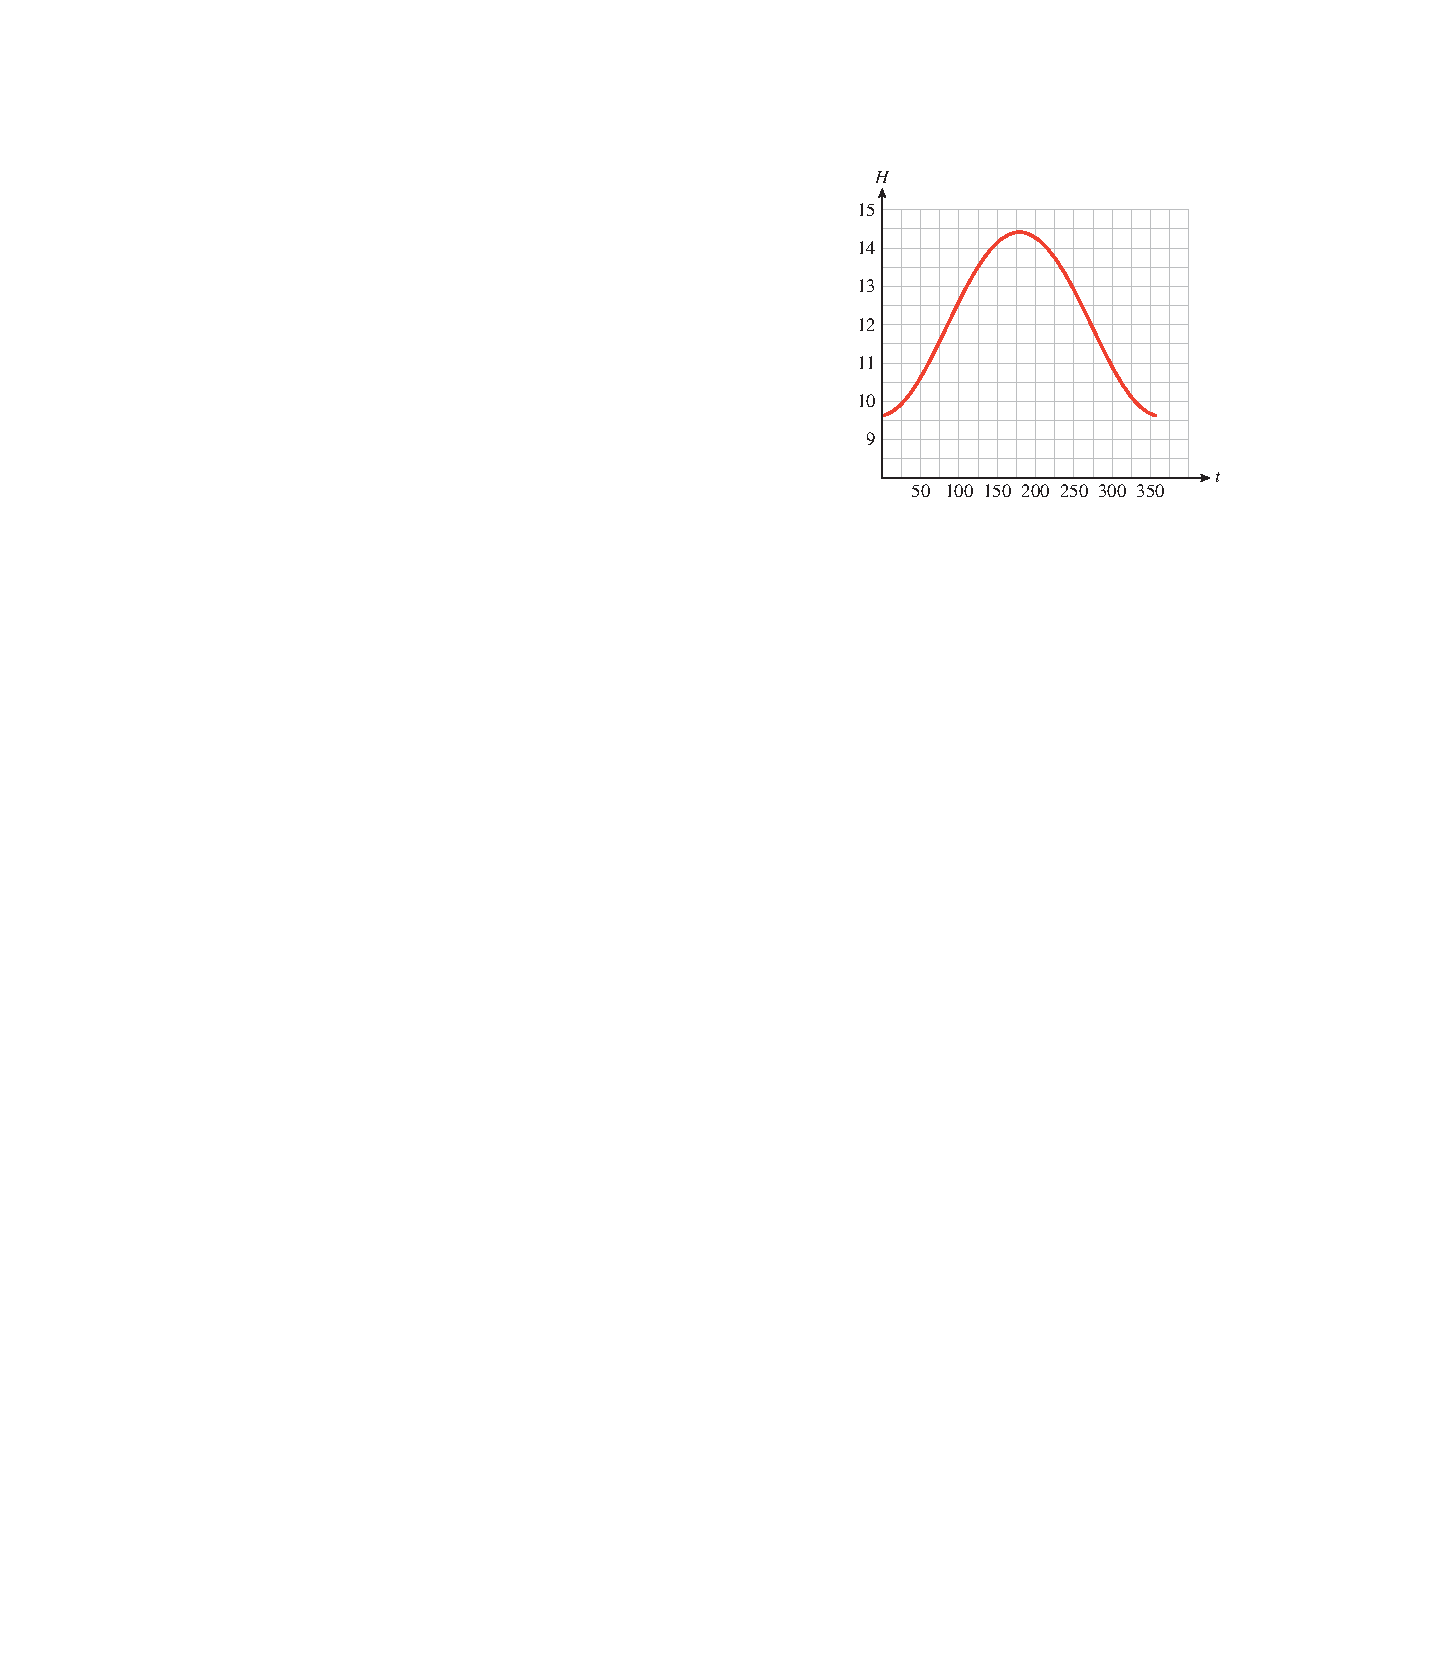
\includegraphics[width=0.5\linewidth]{images/fig-sun-hours}
}
\newlength{\phAimage}\setlength{\phAimage}{\ht\panelboxAimage+\dp\panelboxAimage}
\settototalheight{\phAimage}{\usebox{\panelboxAimage}}
\setlength{\panelmax}{\maxof{\panelmax}{\phAimage}}
\leavevmode%
% begin: side-by-side as figure/tabular
% \tabcolsep change local to group
\setlength{\tabcolsep}{0\textwidth}
% @{} suppress \tabcolsep at extremes, so margins behave as intended
\begin{figure}
\begin{tabular}{@{}*{2}{c}@{}}
\begin{minipage}[c][\panelmax][t]{0.5\textwidth}\usebox{\panelboxAparagraphs}\end{minipage}&
\begin{minipage}[c][\panelmax][t]{0.5\textwidth}\usebox{\panelboxAimage}\end{minipage}\tabularnewline
&
\parbox[t]{0.5\textwidth}{\captionof{figure}{\label{fig-sun-hours}}
}\end{tabular}
\end{figure}
% end: side-by-side as tabular/figure
}% end: group for a single side-by-side
\par\medskip\noindent%
\textbf{Solution.}\quad \leavevmode%
\begin{enumerate}[label=\alph*]
\item\hypertarget{li-19}{}The input variable, \(t\), appears on the horizontal axis. The number of daylight hours, \(H\), is a function of the date. The output variable appears on the vertical axis.%
\item\hypertarget{li-20}{}The point on the curve where \(t = 150\) has \(H \approx 14.1\), so Peoria gets about 14.1 hours of daylight when \(t = 150\), which is at the end of May.%
\item\hypertarget{li-21}{}\(H = 12\) at the two points where \(t \approx 85\) (in late March) and \(t \approx 270\) (late September).%
\item\hypertarget{li-22}{}The maximum value of 14.4 hours occurs on the longest day of the year, when \(t \approx 170\), about three weeks into June. The minimum of 9.6 hours occurs on the shortest day, when \(t \approx 355\), about three weeks into December.%
\end{enumerate}
\end{example}
\begin{exercise}\label{exercise-LA-marathon}
\hyperref[fig-LA-marathon]{Figure~\ref{fig-LA-marathon}}  shows the elevation in feet, \(a\), of the Los Angeles Marathon course at a distance \(d\) miles into the race. (Source: \emph{Los Angeles Times}, March 3, 2005) \begin{figure}
\centering
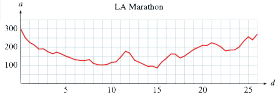
\includegraphics[width=1\linewidth]{images/fig-LA-marathon}
\caption{\label{fig-LA-marathon}}
\end{figure}
\leavevmode%
\begin{enumerate}[label=\alph*]
\item\hypertarget{li-23}{}Which variable is the input, and which is the output?%
\item\hypertarget{li-24}{}What is the elevation at mile 20?%
\item\hypertarget{li-25}{}At what distances is the elevation 150 feet?%
\item\hypertarget{li-26}{}What are the maximum and minimum values of \(a\), and when do these values occur?%
\item\hypertarget{li-27}{}The runners pass by the Los Angeles Coliseum at about 4.2 miles into the race. What is the elevation there?%
\end{enumerate}
\end{exercise}
\typeout{************************************************}
\typeout{Subsection 1.1.4 Functions Defined by Equations}
\typeout{************************************************}
\subsection[{Functions Defined by Equations}]{Functions Defined by Equations}\label{subsection-4}
\hyperref[example-falling-book]{Example~\ref{example-falling-book}} illustrates a function defined by an equation.%
\begin{example}[]\label{example-falling-book}
As of 2016,  One World Trade Center in New York City is the nation’s tallest building, at 1776 feet. If an algebra book is dropped from the top of the Sears Tower, its height above the ground after \(t\) seconds is given by the equation%
\begin{equation*}
h = 1776 - 16t^2
\end{equation*}
Thus, after \(\alert{1}\) second the book’s height is%
\begin{equation*}
h = 1776 - 16(\alert{1})^2 = 1760 \text{ feet}
\end{equation*}
After \(\alert{2}\) seconds its height is%
\begin{equation*}
h = 1776 - 16(\alert{2})^2 = 1712 \text{ feet}
\end{equation*}
For this function, \(t\) is the input variable and \(h\) is the output variable. For any value of \(t\), a unique value of \(h\) can be determined from the equation for \(h\). We say that \(h\) \emph{is a function of} \(t\).%
\end{example}
\begin{exercise}\label{exercise-4}
Write an equation that gives the volume, \(V\), of a sphere as a function of its radius, \(r\).\end{exercise}
\begin{remark}[Making a Table of Values with a Calculator]\label{remark-1}
We can use a graphing calculator to make a table of values for a function defined by an equation. For the function in \hyperref[example-falling-book]{Example~\ref{example-falling-book}},%
\begin{equation*}
h = 1776 - 16t^2
\end{equation*}
we begin by entering the equation: Press the \lstinline?Y=? key, clear out any other equations, and define \(Y_1 = 1776 - 16X^2.\)%
\par
Next, we choose the \(x\)-values for the table. Press \lstinline?2nd?\lstinline?WINDOW? to access the TblSet (Table Setup) menu and set it to look like \hyperref[fig-TblSetup]{Figure~\ref{fig-TblSetup}}. This setting will give us an initial x-value of 0 \((TblStart = 0)\) and an increment of one unit in the x-values, \((\Delta Tbl = 1)\). It also fills in values of both variables automatically. Now press \lstinline?2nd? \lstinline?GRAPH? to see the table of values, as shown in \hyperref[fig-GC-table]{Figure~\ref{fig-GC-table}}. From this table, we can check the heights we found in \hyperref[example-falling-book]{Example~\ref{example-falling-book}}.%
\par
Now try making a table of values with \(TblStart = 0\) and \(\Delta Tbl = 0.5\). Use the  \(\keystroke{ $\uparrow$}\) and \lstinline?↓? arrow keys to scroll up and down the table.%
% group protects changes to lengths, releases boxes (?)
{% begin: group for a single side-by-side
% set panel max height to practical minimum, created in preamble
\setlength{\panelmax}{0pt}
\newsavebox{\panelboxCimage}
\savebox{\panelboxCimage}{%
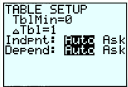
\includegraphics[width=0.5\linewidth]{images/fig-TblSetup}
}
\newlength{\phCimage}\setlength{\phCimage}{\ht\panelboxCimage+\dp\panelboxCimage}
\settototalheight{\phCimage}{\usebox{\panelboxCimage}}
\setlength{\panelmax}{\maxof{\panelmax}{\phCimage}}
\newsavebox{\panelboxDimage}
\savebox{\panelboxDimage}{%
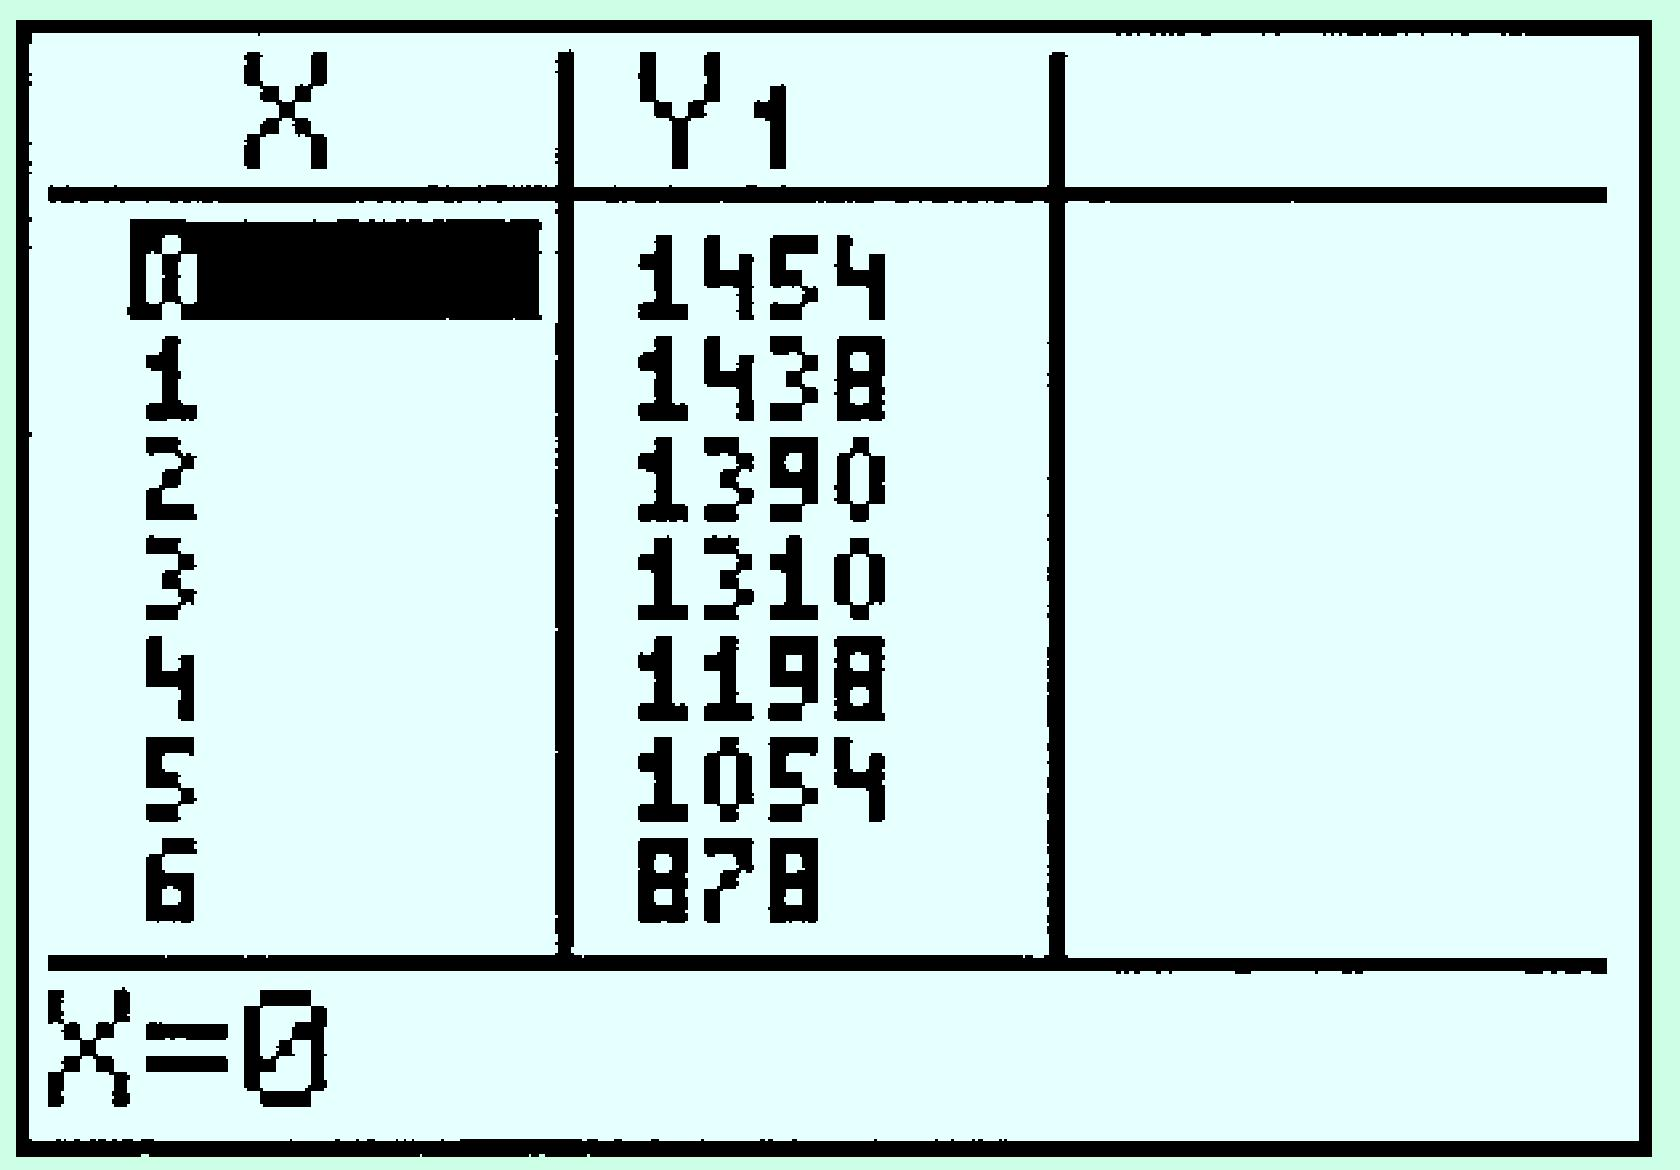
\includegraphics[width=0.5\linewidth]{images/fig-GC-table}
}
\newlength{\phDimage}\setlength{\phDimage}{\ht\panelboxDimage+\dp\panelboxDimage}
\settototalheight{\phDimage}{\usebox{\panelboxDimage}}
\setlength{\panelmax}{\maxof{\panelmax}{\phDimage}}
\leavevmode%
% begin: side-by-side as figure/tabular
% \tabcolsep change local to group
\setlength{\tabcolsep}{0\textwidth}
% @{} suppress \tabcolsep at extremes, so margins behave as intended
\begin{figure}
\begin{tabular}{@{}*{2}{c}@{}}
\begin{minipage}[c][\panelmax][t]{0.5\textwidth}\usebox{\panelboxCimage}\end{minipage}&
\begin{minipage}[c][\panelmax][t]{0.5\textwidth}\usebox{\panelboxDimage}\end{minipage}\tabularnewline
\parbox[t]{0.5\textwidth}{\captionof{figure}{\label{fig-TblSetup}}
}&
\parbox[t]{0.5\textwidth}{\captionof{figure}{\label{fig-GC-table}}
}\end{tabular}
\end{figure}
% end: side-by-side as tabular/figure
}% end: group for a single side-by-side
\end{remark}
\typeout{************************************************}
\typeout{Subsection 1.1.5 Function Notation}
\typeout{************************************************}
\subsection[{Function Notation}]{Function Notation}\label{subsection-5}
There is a convenient notation for discussing functions. First, we choose a letter, such as \(f\), \(g\), or \(h\) (or \(F\), \(G\), or \(H\)), to name a particular function. (We can use any letter, but these are the most common choices.) For instance, in \hyperref[example-falling-book]{Example~\ref{example-falling-book}}, the height, \(h\), of a falling algebra book is a function of the elapsed time, \(t\). We might call this function \(f\). In other words, \(f\) is the name of the relationship between the variables \(h\) and \(t\). We write%
\begin{equation*}
h = f (t)
\end{equation*}
which means "\(h\) is a function of \(t\), and \(f\) is the name of the function."%
\par
The new symbol \(f(t)\), read "\(f\) of \(t\)," is another name for the height, \(h\). The parentheses in the symbol \(f(t)\) do not indicate multiplication. (It would not make sense to multiply the name of a function by a variable.) Think of the symbol \(f(t)\) as a single variable that represents the output value of the function.%
\par
With this new notation we may write%
\begin{equation*}
h = f (t) = 1776 - 16t^2
\end{equation*}
or just%
\begin{equation*}
f (t) = 1776 - 16t^2
\end{equation*}
instead of%
\begin{equation*}
h = 1776 - 16t^2
\end{equation*}
to describe the function.%
\par
Perhaps it seems complicated to introduce a new symbol for \(h\), but the notation \(f(t)\) is very useful for showing the correspondence between specific values of the variables \(h\) and \(t\).%
\begin{example}[]\label{example-falling-book-2}
In \hyperref[example-falling-book]{Example~\ref{example-falling-book}}, the height of an algebra book dropped from the top of the Sears Tower is given by the equation%
\begin{equation*}
h = 1776 - 16t^2
\end{equation*}
We see that%
\begin{table}
\centering
\begin{tabular}{lll}
when \(t=1\)&&\(h=1760\)\tabularnewline[0pt]
when \(t=2\)&&\(h=1712\)
\end{tabular}
\end{table}
Using function notation, these relationships can be expressed more concisely as%
\begin{table}
\centering
\begin{tabular}{lll}
\(f(1)=1760\)&and&\(f(2)=1712\)
\end{tabular}
\end{table}
which we read as "\(f\) of 1 equals 1760" and "\(f\) of 2 equals 1712." The values for the input variable, \(t\), appear \emph{inside} the parentheses, and the values for the output variable, \(h\), appear on the other side of the equation.%
\end{example}
Remember that when we write \(y = f(x)\), the symbol \(f(x)\) is just another name for the output variable.%
\begin{assemblage}{Function Notation}\label{assemblage-2}
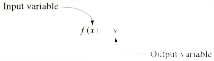
\includegraphics[width=0.7\linewidth]{images/fig-Function-Notation}
%
\end{assemblage}
\begin{exercise}\label{exercise-5}
Let \(F\) be the name of the function defined by the graph in \hyperref[example-sun-hours]{Example~\ref{example-sun-hours}}, the number of hours of daylight in Peoria. \leavevmode%
\begin{enumerate}[label=\alph*]
\item\hypertarget{li-33}{}Use function notation to state that \(H\) is a function of \(t\).%
\item\hypertarget{li-34}{}What does the statement \(F(15) = 9.7\) mean in the context of the problem?%
\end{enumerate}
\end{exercise}
\typeout{************************************************}
\typeout{Subsection 1.1.6 Evaluating a Function}
\typeout{************************************************}
\subsection[{Evaluating a Function}]{Evaluating a Function}\label{subsection-6}
Finding the value of the output variable that corresponds to a particular value of the input variable is called \terminology{evaluating the function}.%
\begin{example}[]\label{example-postage2}
Let \(g\) be the name of the postage function defined by \hyperref[table-postage]{Table~\ref{table-postage}}  in \hyperref[example-functions]{Example~\ref{example-functions}}. Find \(g(1)\), \(g(3)\), and \(g(6.75\)).%
\par\medskip\noindent%
\textbf{Solution.}\quad According to the table, \leavevmode%
\begin{table}
\centering
\begin{tabular}{lllll}
when \(w=1\),&&\(p=0.47\)&so&\(g(1)=0.47\)\tabularnewline[0pt]
when \(w=3\),&&\(p=0.89\)&so&\(g(3)=0.89\)\tabularnewline[0pt]
when \(w=6.75\),&&\(p=1.73\)&so&\(g(6.75)=1.73\)
\end{tabular}
\end{table}
 Thus, a letter weighing 1 ounce costs \textdollar{}0.47 to mail, a letter weighing 3 ounces costs \textdollar{}0.89, and a letter weighing 6.75 ounces costs \textdollar{}1.73.%
\end{example}
\begin{exercise}\label{exercise-heart-rate}
When you exercise, your heart rate should increase until it reaches your target heart rate. The table shows target heart rate, \(r = f(a)\), as a function of age. \begin{table}
\centering
\begin{tabular}{AcAcAcAcAcAcAcAcAcAcAcAcA}\hrulethick
\(a\)&\(20\)&\(25\)&\(30\)&\(35\)&\(40\)&\(45\)&\(50\)&\(55\)&\(60\)&\(65\)&\(70\)\tabularnewline\hrulethin
\(r\)&\(150\)&\(146\)&\(142\)&\(139\)&\(135\)&\(131\)&\(127\)&\(124\)&\(120\)&\(116\)&\(112\)\tabularnewline\hrulethin
\end{tabular}
\end{table}
\leavevmode%
\begin{enumerate}[label=\alph*]
\item\hypertarget{li-37}{}Find \(f(25)\) and \(f(50)\).%
\item\hypertarget{li-38}{}Find a value of \(a\) for which \(f(a) = 135\).%
\end{enumerate}
\end{exercise}
If a function is described by an equation, we simply substitute the given input value into the equation to find the corresponding output, or function value.%
\begin{example}[]\label{example-evaluate-function}
The function \(H\) is defined by \(H=f(s) = \dfrac{\sqrt{s+3}}{s}\). Evaluate the function at the following values.%
\leavevmode%
\begin{enumerate}[label=\alph*]
\item\hypertarget{li-41}{}\(s=6\)%
\item\hypertarget{li-42}{}\(s=-1\)%
\end{enumerate}
\par\medskip\noindent%
\textbf{Solution.}\quad \leavevmode%
\begin{enumerate}[label=\alph*]
\item\hypertarget{li-43}{}\(f(\alert{6})=\frac{\sqrt{\alert{6}+3}}{\alert{6}}=
\frac{\sqrt{9}}{6}=\frac{3}{6}=\frac{1}{2}\). Thus, \(f(6)=\frac{1}{2}\).%
\item\hypertarget{li-44}{}\(f(\alert{-1})=\frac{\sqrt{\alert{-1}+3}}{\alert{-1}}=
\frac{\sqrt{2}}{-1}=-\sqrt{2}\). Thus, \(f(-1)=-\sqrt{2}\).%
\end{enumerate}
\end{example}
\begin{exercise}\label{exercise-function-notation}
Complete the table displaying ordered pairs for the function \(f(x) = 5 - x^3\). Evaluate the function to find the corresponding \(f(x)\)-value for each value of \(x\). \begin{table}
\centering
\begin{tabular}{AcAcAl}\crulethick{1-2}
\(x\)&\(f(x)\)&\tabularnewline\crulethin{1-2}
\(-2\)&\(\)&\(f(\alert{-2})=5-(\alert{-2})^3=~\)\tabularnewline\crulethin{1-2}
\(0\)&\(\)&\(f(\alert{0})=5-\alert{0}^3=\)\tabularnewline\crulethin{1-2}
\(1\)&\(\)&\(f(\alert{1})=5-\alert{1}^3=\)\tabularnewline\crulethin{1-2}
\(3\)&\(\)&\(f(\alert{3})=5-\alert{3}^3=\)\tabularnewline\crulethin{1-2}
\end{tabular}
\end{table}
\end{exercise}
\begin{remark}[Evaluating a Function]\label{remark-2}
We can use the table feature on a graphing calculator to evaluate functions. Consider the function of \hyperref[exercise-function-notation]{Exercise~\ref{exercise-function-notation}}, \(f(x) = 5 - x^3\).%
\par
Press \lstinline?Y=?, clear any old functions, and enter%
\begin{equation*}
Y_1 = 5-X \text{^} 3
\end{equation*}
Then press TblSet (\lstinline?2nd? \lstinline?WINDOW?) and choose Ask after Indpnt, as shown in \hyperref[fig-TblSetup2]{Figure~\ref{fig-TblSetup2}}, and press \lstinline?ENTER?. This setting allows you to enter any \(x\)-values you like. Next, press TABLE (using \lstinline?2nd? \lstinline?GRAPH?).%
\par
To follow \hyperref[exercise-function-notation]{Exercise~\ref{exercise-function-notation}}, key in \lstinline?(-)? 2 \lstinline?ENTER? for the \(x\)-value, and the calculator will fill in the \(y\)-value. Continue by entering 0, 1, 3, or any other \(x\)-values you choose. One such table is shown in \hyperref[fig-GC-table2]{Figure~\ref{fig-GC-table2}}.%
\par
If you would like to evaluate a new function, you do not have to return to the \lstinline?Y=? screen. Use the \lstinline?→? and \lstinline?↑? arrow keys to highlight \(Y_1\) at the top of the second column. The definition of \(Y_1\) will appear at the bottom of the display, as shown in \hyperref[fig-GC-table2]{Figure~\ref{fig-GC-table2}}. You can key in a new definition here, and the second column will be updated automatically to show the \(y\)-values of the new function. % group protects changes to lengths, releases boxes (?)
{% begin: group for a single side-by-side
% set panel max height to practical minimum, created in preamble
\setlength{\panelmax}{0pt}
\newsavebox{\panelboxFimage}
\savebox{\panelboxFimage}{%
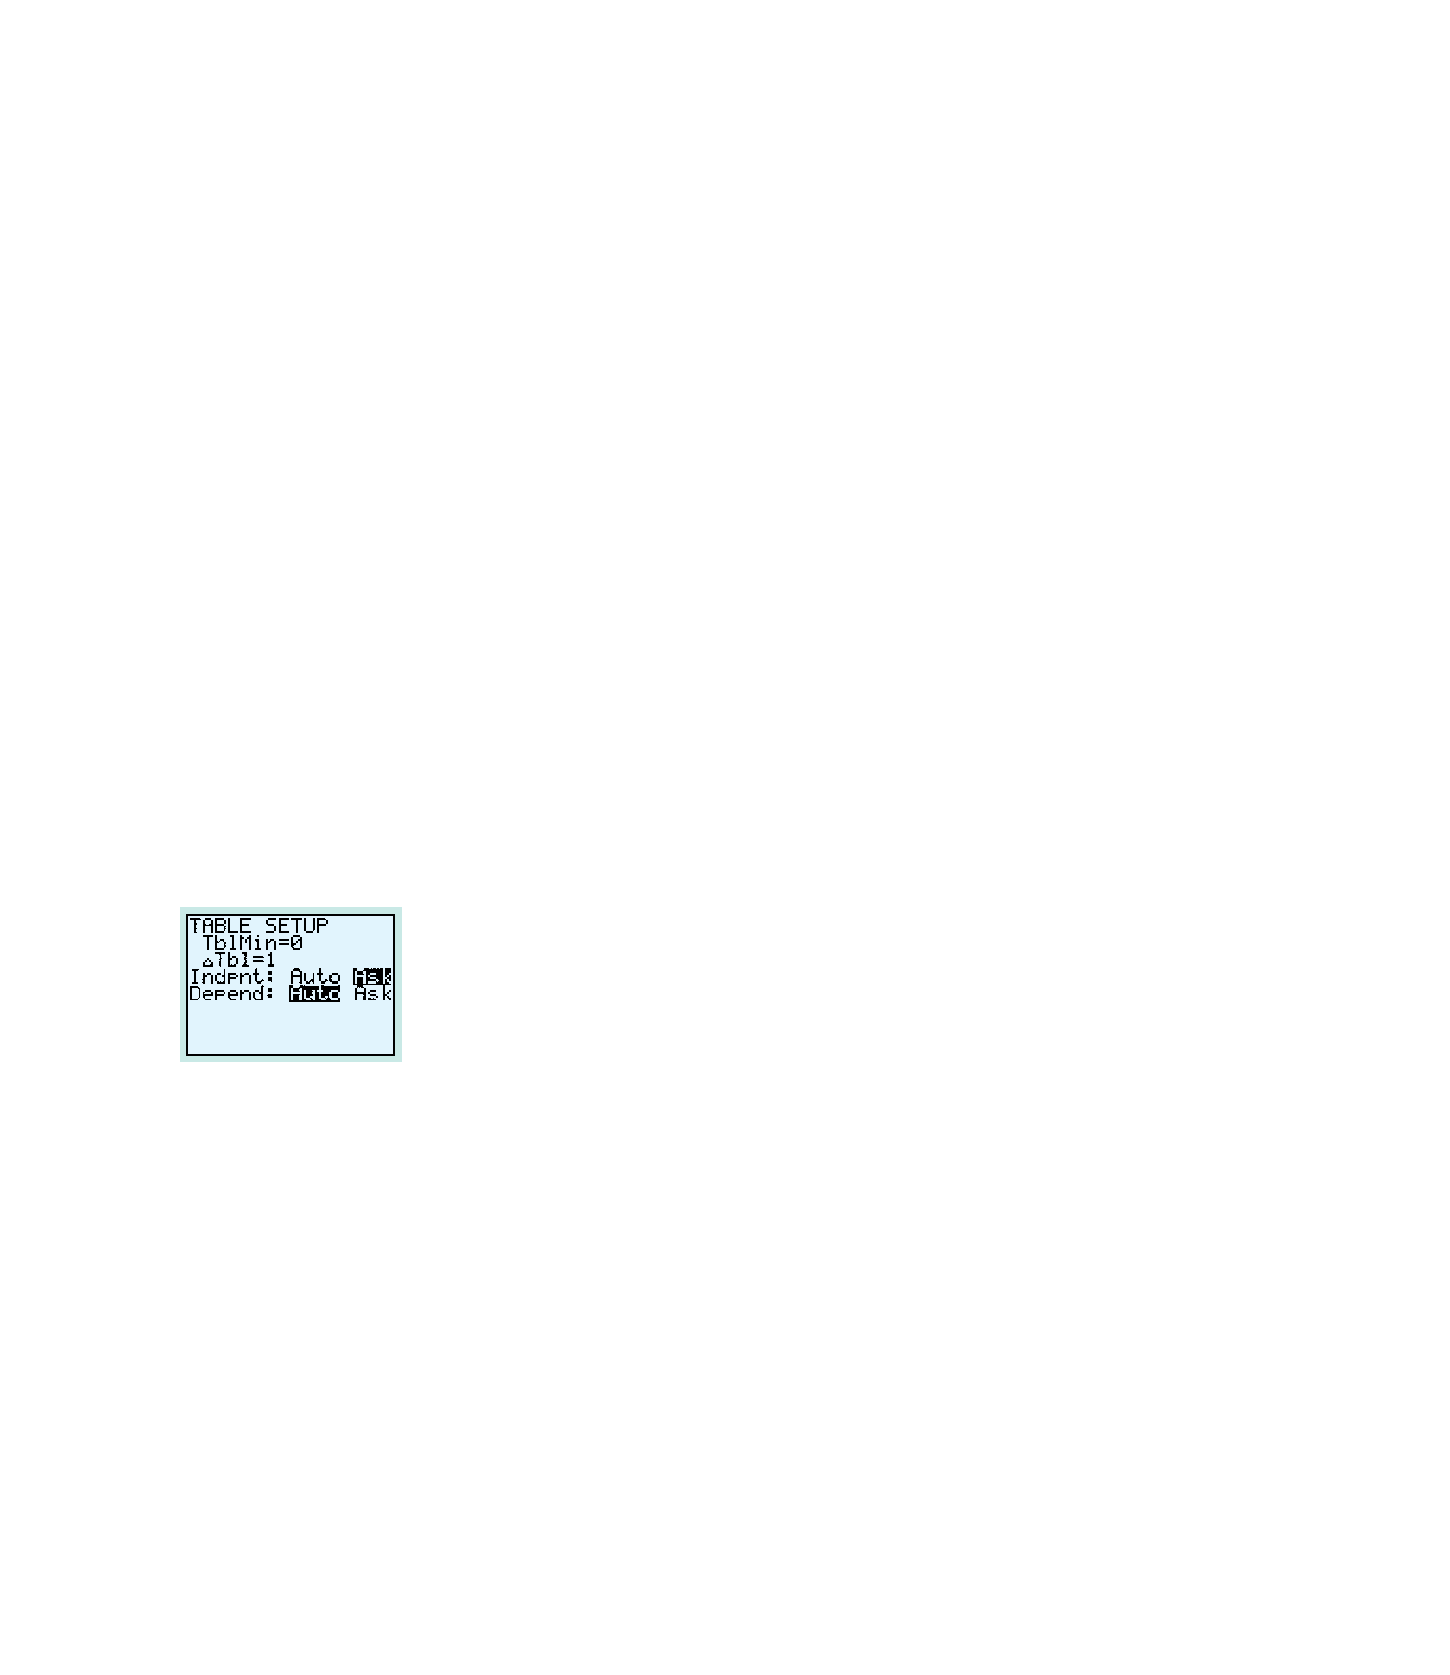
\includegraphics[width=0.5\linewidth]{images/fig-TblSetup2}
}
\newlength{\phFimage}\setlength{\phFimage}{\ht\panelboxFimage+\dp\panelboxFimage}
\settototalheight{\phFimage}{\usebox{\panelboxFimage}}
\setlength{\panelmax}{\maxof{\panelmax}{\phFimage}}
\newsavebox{\panelboxGimage}
\savebox{\panelboxGimage}{%
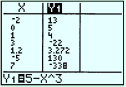
\includegraphics[width=0.5\linewidth]{images/fig-GC-table2}
}
\newlength{\phGimage}\setlength{\phGimage}{\ht\panelboxGimage+\dp\panelboxGimage}
\settototalheight{\phGimage}{\usebox{\panelboxGimage}}
\setlength{\panelmax}{\maxof{\panelmax}{\phGimage}}
\leavevmode%
% begin: side-by-side as figure/tabular
% \tabcolsep change local to group
\setlength{\tabcolsep}{0\textwidth}
% @{} suppress \tabcolsep at extremes, so margins behave as intended
\begin{figure}
\begin{tabular}{@{}*{2}{c}@{}}
\begin{minipage}[c][\panelmax][t]{0.5\textwidth}\usebox{\panelboxFimage}\end{minipage}&
\begin{minipage}[c][\panelmax][t]{0.5\textwidth}\usebox{\panelboxGimage}\end{minipage}\tabularnewline
\parbox[t]{0.5\textwidth}{\captionof{figure}{\label{fig-TblSetup2}}
}&
\parbox[t]{0.5\textwidth}{\captionof{figure}{\label{fig-GC-table2}}
}\end{tabular}
\end{figure}
% end: side-by-side as tabular/figure
}% end: group for a single side-by-side
%
\end{remark}
To simplify the notation, we sometimes use the same letter for the output variable and for the name of the function. In the next example, \(C\) is used in this way.%
\begin{example}[]\label{example-function-notation-abuse}
TrailGear decides to market a line of backpacks. The cost, \(C\), of manufacturing backpacks is a function of the number, \(x\), of backpacks produced, given by the equation%
\begin{equation*}
C(x) = 3000 + 20x
\end{equation*}
where \(C(x)\) is measured in dollars. Find the cost of producing 500 backpacks.%
\par\medskip\noindent%
\textbf{Solution.}\quad To find the value of \(C\) that corresponds to \(x = \alert{500}\), evaluate \(C(500)\).%
\begin{equation*}
C(\alert{500}) = 3000 + 20(\alert{500}) = 13,000
\end{equation*}
The cost of producing 500 backpacks is \textdollar{}13,000.%
\end{example}
\begin{exercise}\label{exercise-sphere-volume}
The volume of a sphere of radius \(r\) centimeters is given by%
\begin{equation*}
V = V(r) = \frac{4}{3}\pi r^3
\end{equation*}
Evaluate \(V(10)\) and explain what it means.%
\end{exercise}
\typeout{************************************************}
\typeout{Subsection 1.1.7 Operations with Function Notation}
\typeout{************************************************}
\subsection[{Operations with Function Notation}]{Operations with Function Notation}\label{subsection-7}
Sometimes we need to evaluate a function at an algebraic expression rather than at a specific number.%
\begin{example}[]\label{example-backpacks}
TrailGear manufactures backpacks at a cost of%
\begin{equation*}
C(x) = 3000 + 20x
\end{equation*}
for \(x\) backpacks. The company finds that the monthly demand for backpacks increases by 50% during the summer. The backpacks are produced at several small co-ops in different states.%
\leavevmode%
\begin{enumerate}[label=\alph*]
\item\hypertarget{li-45}{}If each co-op usually produces \(b\) backpacks per month, how many should it produce during the summer months?%
\item\hypertarget{li-46}{}What costs for producing backpacks should the company expect during the summer?%
\end{enumerate}
\par\medskip\noindent%
\textbf{Solution.}\quad \leavevmode%
\begin{enumerate}[label=\alph*]
\item\hypertarget{li-47}{}An increase of 50% means an additional 50% of the current production level, \(b\). Therefore, a co-op that produced \(b\) backpacks per month during the winter should increase production to \(b + 0.5b\), or \(1.5b\) backpacks per month in the summer.%
\item\hypertarget{li-48}{}The cost of producing \(1.5b\) backpacks will be%
\begin{equation*}
C(\alert{1.5b}) = 3000 + 20(\alert{1.5b}) = 3000 + 30b
\end{equation*}
%
\end{enumerate}
\end{example}
\begin{exercise}\label{exercise-spherical-balloon}
A spherical balloon has a radius of 10 centimeters. \leavevmode%
\begin{enumerate}[label=\alph*]
\item\hypertarget{li-49}{}If we increase the radius by \(h\) centimeters, what will the new volume be?%
\item\hypertarget{li-50}{}If \(h = 2\), how much did the volume increase?%
\end{enumerate}
\end{exercise}
\begin{example}[]\label{example-evaluate-quadratic}
Evaluate the function \(f(x)=4x^2 - x + 5\) for the following expressions.%
\leavevmode%
\begin{enumerate}[label=\alph*]
\item\hypertarget{li-53}{}\(x = 2h\)%
\item\hypertarget{li-54}{}\(x = a + 3\)%
\end{enumerate}
\par\medskip\noindent%
\textbf{Solution.}\quad \leavevmode%
\begin{enumerate}[label=\alph*]
\item\hypertarget{li-55}{}~%
\par
\(\begin{aligned}
f(\alert{2h}) \amp= 4(\alert{2h})^2-(\alert{2h}) + 5\\
\amp= 4(4h^2)-2h+5\\
\amp= 16h^2 - 2h + 5\\ 
\end{aligned}\)%
\item\hypertarget{li-56}{}~%
\par
\(\begin{aligned}
f(\alert{a+3}) \amp= 4(\alert{a+3})^2-(\alert{a+3})+5\\
\amp= 4(a^2+6a+9)-a-3+5\\
\amp= 4a^2+24a+36 - a + 2\\
\amp= 4a^2+23a + 38\\
\end{aligned}\)%
\end{enumerate}
\end{example}
\typeout{************************************************}
\typeout{Paragraphs  CAUTION}
\typeout{************************************************}
\paragraph[{CAUTION}]{CAUTION}\hypertarget{paragraphs-2}{}
In \hyperref[example-evaluate-quadratic]{Example~\ref{example-evaluate-quadratic}}, notice that%
\begin{equation*}
f(2h) \ne 2 f(h)
\end{equation*}
and%
\begin{equation*}
f(a + 3) \ne f(a) + f(3)
\end{equation*}
To compute \(f(a) + f(3)\), we must first compute \(f(a)\) and \(f(3)\), then add them: \begin{align*} f(a)+f(3)\&= (4a^2-a+5)+(4\cdot 3^2-3+5) \textbackslash{}\textbackslash{} \&= 4a^2 - a + 43\textbackslash{}\textbackslash{} \end{align*} In general, it is not true that \(f(a + b) = f(a) + f(b)\). Remember that the parentheses in the expression \(f(x)\) do not indicate multiplication, so the distributive law does not apply to the expression \(f(a + b)\).%
\begin{exercise}\label{exercise-function-notation2}
Let \(f(x) = x^3 - 1\) and evaluate each expression. \leavevmode%
\begin{enumerate}[label=\alph*]
\item\hypertarget{li-57}{}\(f(2) + f(3)\)%
\item\hypertarget{li-58}{}\(f(2 + 3)\)%
\item\hypertarget{li-59}{}\(2 f(x) + 3\)%
\end{enumerate}
\end{exercise}
\typeout{************************************************}
\typeout{Subsection 1.1.8 Section Summary}
\typeout{************************************************}
\subsection[{Section Summary}]{Section Summary}\label{summary-1-2}
\typeout{************************************************}
\typeout{Subsubsection 1.1.8.1 Vocabulary}
\typeout{************************************************}
\subsubsection[{Vocabulary}]{Vocabulary}\label{subsubsection-1}
Look up the definitions of new terms in the Glossary. \leavevmode%
\begin{multicols}{3}
\begin{itemize}[label=\textbullet]
\item{}Function%
\item{}Input variable%
\item{}Independent variable%
\item{}Dependent variable%
\item{}Function value%
\item{}Output variable%
\end{itemize}
\end{multicols}
%
\typeout{************************************************}
\typeout{Subsubsection 1.1.8.2 CONCEPTS}
\typeout{************************************************}
\subsubsection[{CONCEPTS}]{CONCEPTS}\label{subsubsection-2}
\leavevmode%
\begin{enumerate}[label=\arabic*]
\item\hypertarget{li-69}{}A function is a rule that assigns to each value of the input variable a unique value of the output variable.%
\item\hypertarget{li-70}{}Functions may be defined by words, tables, graphs, or equations.%
\item\hypertarget{li-71}{}Function notation: \(y = f (x)\), where \(x\) is the input and \(y\) is the output.%
\end{enumerate}
%
\typeout{************************************************}
\typeout{Subsubsection 1.1.8.3 STUDY QUESTIONS}
\typeout{************************************************}
\subsubsection[{STUDY QUESTIONS}]{STUDY QUESTIONS}\label{subsubsection-3}
\leavevmode%
\begin{enumerate}[label=\arabic*]
\item\hypertarget{li-72}{}What property makes a relation between two variables a function?%
\item\hypertarget{li-73}{}Name three ways to define a function.%
\item\hypertarget{li-74}{}Give an example of a function in which two distinct values of the input variable correspond to the same value of the output variable.%
\item\hypertarget{li-75}{}Use function notation to write the statement "\(G\) defines \(w\) as a function of \(p\)."%
\item\hypertarget{li-76}{}Give an example of a function for which \(f (2 + 3)\ne f (2) + f (3)\).%
\end{enumerate}
%
\typeout{************************************************}
\typeout{Subsubsection 1.1.8.4 SKILLS}
\typeout{************************************************}
\subsubsection[{SKILLS}]{SKILLS}\label{subsubsection-4}
Practice each skill in the \hyperref[section-1-2-exercises]{Homework~\ref{section-1-2-exercises}} problems listed. \leavevmode%
\begin{enumerate}[label=\arabic*]
\item\hypertarget{li-77}{}Decide whether a relationship between two variables is a function: \#1\textendash{}26%
\item\hypertarget{li-78}{}Evaluate a function defined by a table, a graph, or an equation: \#27\textendash{}54%
\item\hypertarget{li-79}{}Choose appropriate scales for the axes: \#5\textendash{}12%
\item\hypertarget{li-80}{}Interpret function notation: \#31\textendash{}34, 49\textendash{}54%
\item\hypertarget{li-81}{}Simplify expressions involving function notation: \#59\textendash{}76%
\end{enumerate}
%
\typeout{************************************************}
\typeout{Exercises 1.1.9 Homework}
\typeout{************************************************}
\subsection[{Homework}]{Homework}\label{section-1-2-exercises}
\hypertarget{exercisegroup-1}{}\par\noindent For which of the following pairs is the second quantity a function of the first? Explain your answers.%
\begin{exercisegroup}(1)
\exercise[1.]\hypertarget{exercise-11}{}Price of an item; sales tax on the item at 4\%%
\par\smallskip
\noindent\textbf{Answer.}\hypertarget{answer-11}{}\quad
Function; the tax is determined by the price of the item.%
\exercise[2.]\hypertarget{exercise-12}{}Time traveled at constant speed; distance traveled%
\exercise[3.]\hypertarget{exercise-13}{}Number of years of education; annual income%
\par\smallskip
\noindent\textbf{Answer.}\hypertarget{answer-12}{}\quad
Not a function; incomes may differ for same number of years of education.%
\exercise[4.]\hypertarget{exercise-14}{}Distance flown in an airplane; price of the ticket%
\exercise[5.]\hypertarget{exercise-15}{}Volume of a container of water; the weight of the water%
\par\smallskip
\noindent\textbf{Answer.}\hypertarget{answer-13}{}\quad
Function; weight is determined by volume.%
\exercise[6.]\hypertarget{exercise-16}{}Amount of a paycheck; amount of Social Security tax withheld%
\end{exercisegroup}
\par\smallskip\noindent
\hypertarget{exercisegroup-2}{}\par\noindent Each of the following objects establishes a correspondence between two variables. Suggest appropriate input and output variables and decide whether the relationship is a function.%
\begin{exercisegroup}(2)
\exercise[7.]\hypertarget{exercise-17}{}An itemized grocery receipt%
\par\smallskip
\noindent\textbf{Answer.}\hypertarget{answer-14}{}\quad
Input: items purchased; output: price of item. Yes, a function because each item has only one price.%
\exercise[8.]\hypertarget{exercise-18}{}An inventory list%
\exercise[9.]\hypertarget{exercise-19}{}An index%
\par\smallskip
\noindent\textbf{Answer.}\hypertarget{answer-15}{}\quad
Input: topics; output: page or pages on which topic occurs. No, not a function because the same topic may appear in more than one page.%
\exercise[10.]\hypertarget{exercise-20}{}A will%
\exercise[11.]\hypertarget{exercise-21}{}An instructor's grade book%
\par\smallskip
\noindent\textbf{Answer.}\hypertarget{answer-16}{}\quad
Input: students’ names; output: students’ scores on quizzes, tests, etc. No, not a function because the same student can have different grades on different tests.%
\exercise[12.]\hypertarget{exercise-22}{}An address book%
\exercise[13.]\hypertarget{exercise-23}{}A bathroom scale%
\par\smallskip
\noindent\textbf{Answer.}\hypertarget{answer-17}{}\quad
Input: person stepping on scales; output: person's weight. Yes, a function because a person cannot have two different weights at the same time.%
\exercise[14.]\hypertarget{exercise-24}{}A radio dial%
\end{exercisegroup}
\par\smallskip\noindent
\hypertarget{exercisegroup-3}{}\par\noindent Which of the following tables define the second variable as a function of the first variable? Explain why or why not.%
\begin{exercisegroup}(4)
\exercise[15.]\hypertarget{exercise-25}{}\begin{tabular}{AcAcA}\hrulethick
\(x\)&\(t\)\tabularnewline\hrulethin
\(-1\)&\(2\)\tabularnewline\hrulethin
\(0\)&\(9\)\tabularnewline\hrulethin
\(1\)&\(-2\)\tabularnewline\hrulethin
\(0\)&\(-3\)\tabularnewline\hrulethin
\(-1\)&\(5\)\tabularnewline\hrulethin
\end{tabular}
%
\par\smallskip
\noindent\textbf{Answer.}\hypertarget{answer-18}{}\quad
No%
\exercise[16.]\hypertarget{exercise-26}{}\begin{tabular}{AcAcA}\hrulethick
\(y\)&\(w\)\tabularnewline\hrulethin
\(0\)&\(8\)\tabularnewline\hrulethin
\(1\)&\(12\)\tabularnewline\hrulethin
\(3\)&\(7\)\tabularnewline\hrulethin
\(5\)&\(-3\)\tabularnewline\hrulethin
\(7\)&\(4\)\tabularnewline\hrulethin
\end{tabular}
%
\exercise[17.]\hypertarget{exercise-27}{}\begin{tabular}{AcAcA}\hrulethick
\(x\)&\(y\)\tabularnewline\hrulethin
\(-3\)&\(8\)\tabularnewline\hrulethin
\(-2\)&\(3\)\tabularnewline\hrulethin
\(-1\)&\(0\)\tabularnewline\hrulethin
\(0\)&\(-1\)\tabularnewline\hrulethin
\(1\)&\(0\)\tabularnewline\hrulethin
\(2\)&\(3\)\tabularnewline\hrulethin
\(3\)&\(8\)\tabularnewline\hrulethin
\end{tabular}
%
\par\smallskip
\noindent\textbf{Answer.}\hypertarget{answer-19}{}\quad
Yes%
\exercise[18.]\hypertarget{exercise-28}{}\begin{tabular}{AcAcA}\hrulethick
\(s\)&\(t\)\tabularnewline\hrulethin
\(2\)&\(5\)\tabularnewline\hrulethin
\(4\)&\(10\)\tabularnewline\hrulethin
\(6\)&\(15\)\tabularnewline\hrulethin
\(8\)&\(20\)\tabularnewline\hrulethin
\(6\)&\(25\)\tabularnewline\hrulethin
\(4\)&\(30\)\tabularnewline\hrulethin
\(2\)&\(35\)\tabularnewline\hrulethin
\end{tabular}
%
\end{exercisegroup}
\par\smallskip\noindent
\hypertarget{exercisegroup-4}{}\begin{exercisegroup}(2)
\exercise[19.]\hypertarget{exercise-29}{}\begin{tabular}{AcAcAcAcAcAcA}\hrulethick
\(r\)&\(-4\)&\(-2\)&\(0\)&\(2\)&\(4\)\tabularnewline\hrulethin
\(v\)&\(6\)&\(6\)&\(3\)&\(6\)&\(8\)\tabularnewline\hrulethin
\end{tabular}
%
\par\smallskip
\noindent\textbf{Answer.}\hypertarget{answer-20}{}\quad
Yes%
\exercise[20.]\hypertarget{exercise-30}{}\begin{tabular}{AcAcAcAcAcAcA}\hrulethick
\(p\)&\(-5\)&\(-4\)&\(-3\)&\(-2\)&\(-1\)\tabularnewline\hrulethin
\(d\)&\(-5\)&\(-4\)&\(-3\)&\(-2\)&\(-1\)\tabularnewline\hrulethin
\end{tabular}
%
\exercise[21.]\hypertarget{exercise-31}{}\begin{tabular}{AcAcA}\hrulethick
Pressure (\(p\))&Volume (\(v\))\tabularnewline\hrulethin
\(15\)&\(100.0\)\tabularnewline\hrulethin
\(20\)&\(75.0\)\tabularnewline\hrulethin
\(25\)&\(60.0\)\tabularnewline\hrulethin
\(30\)&\(50.0\)\tabularnewline\hrulethin
\(35\)&\(42.8\)\tabularnewline\hrulethin
\(40\)&\(37.5\)\tabularnewline\hrulethin
\(45\)&\(33.3\)\tabularnewline\hrulethin
\(50\)&\(30.0\)\tabularnewline\hrulethin
\end{tabular}
%
\par\smallskip
\noindent\textbf{Answer.}\hypertarget{answer-21}{}\quad
Yes%
\exercise[22.]\hypertarget{exercise-32}{}\begin{tabular}{AcAcA}\hrulethick
Frequency (\(f\))&Wavelength (\(w\))\tabularnewline\hrulethin
\(5\)&\(60.0\)\tabularnewline\hrulethin
\(10\)&\(30.0\)\tabularnewline\hrulethin
\(20\)&\(15.0\)\tabularnewline\hrulethin
\(30\)&\(10.0\)\tabularnewline\hrulethin
\(40\)&\(7.5\)\tabularnewline\hrulethin
\(50\)&\(6.0\)\tabularnewline\hrulethin
\(60\)&\(5.0\)\tabularnewline\hrulethin
\(70\)&\(4.3\)\tabularnewline\hrulethin
\end{tabular}
%
\exercise[23.]\hypertarget{exercise-33}{}\begin{tabular}{AcAcA}\hrulethick
Temperature (\(T\))&Humidity (\(h\))\tabularnewline\hrulethin
Jan. 1 \(34\degree\)F&\(42\%\)\tabularnewline\hrulethin
Jan. 2 \(36\degree\)F&\(44\%\)\tabularnewline\hrulethin
Jan. 3 \(35\degree\)F&\(47\%\)\tabularnewline\hrulethin
Jan. 4 \(29\degree\)F&\(50\%\)\tabularnewline\hrulethin
Jan. 5 \(31\degree\)F&\(52\%\)\tabularnewline\hrulethin
Jan. 6\(35\degree\)F&\(51%\)\tabularnewline\hrulethin
Jan. 7 \(34\degree\)F&\(49\%\)\tabularnewline\hrulethin
\end{tabular}
%
\par\smallskip
\noindent\textbf{Answer.}\hypertarget{answer-22}{}\quad
No%
\exercise[24.]\hypertarget{exercise-34}{}\begin{tabular}{AcAcA}\hrulethick
\tablecelllines{c}{m}
{Inflation\\
rate (\(I\))}
&\tablecelllines{c}{m}
{Unemployment\\
rate (\(U\))}
\tabularnewline\hrulethin
1972 \(\hphantom{000}5.6\%\)&\(5.1\%\)\tabularnewline\hrulethin
1973 \(\hphantom{000}6.2\%\)&\(4.5\%\)\tabularnewline\hrulethin
1974 \(\hphantom{000}10.1\%\)&\(4.9\%\)\tabularnewline\hrulethin
1975 \(\hphantom{000}9.2\%\)&\(7.4\%\)\tabularnewline\hrulethin
1976 \(\hphantom{000}5.8\%\)&\(6.7\%\)\tabularnewline\hrulethin
1977 \(\hphantom{000}5.6\%\)&\(6.8\%\)\tabularnewline\hrulethin
1978 \(\hphantom{000}6.7\%\)&\(7.4\%\)\tabularnewline\hrulethin
\end{tabular}
%
\exercise[25.]\hypertarget{exercise-35}{}\begin{tabular}{AcAcA}\hrulethick
\tablecelllines{c}{m}
{Adjusted gross\\
income (\(I\))}
&Tax bracket (\(T\))\tabularnewline\hrulethin
\(\$0-2479\)&\(0\%\)\tabularnewline\hrulethin
\(\$2480-3669\)&\(4.5\%\)\tabularnewline\hrulethin
\(\$3670-4749\)&\(12\%\)\tabularnewline\hrulethin
\(\$4750-7009\)&\(14\%\)\tabularnewline\hrulethin
\(\$7010-9169\)&\(15\%\)\tabularnewline\hrulethin
\($9170-11,649\)&\(16\%\)\tabularnewline\hrulethin
\($11,650-13,919\)&\(18\%\)\tabularnewline\hrulethin
\end{tabular}
%
\par\smallskip
\noindent\textbf{Answer.}\hypertarget{answer-23}{}\quad
Yes%
\exercise[26.]\hypertarget{exercise-36}{}\begin{tabular}{AcAcA}\hrulethick
\tablecelllines{c}{m}
{Cost of\\
merchandise (\(M\))}
&\tablecelllines{c}{m}
{Shipping\\
charge  (\(C\))}
\tabularnewline\hrulethin
\(\$0.01-10.00\)&\(\$2.50\)\tabularnewline\hrulethin
\(10.01-20.00\)&\(3.75\)\tabularnewline\hrulethin
\(20.01-35.00\)&\(4.85\)\tabularnewline\hrulethin
\(30.01-50.00\)&\(5.95\)\tabularnewline\hrulethin
\(50.01-75.00\)&\(6.95\)\tabularnewline\hrulethin
\(75.01-100.00\)&\(7.95\)\tabularnewline\hrulethin
Over \(100.00\)&\(8.95\)\tabularnewline\hrulethin
\end{tabular}
%
\end{exercisegroup}
\par\smallskip\noindent
\begin{exerciselist}
\item[27.]\hypertarget{exercise-37}{}The function described in Problem 21 is called \(g\), so that \(v = g( p)\). Find the following: \leavevmode%
\begin{enumerate}[label=\alph*]
\item\hypertarget{li-82}{}\(g(25)\)%
\item\hypertarget{li-83}{}\(g(40)\)%
\item\hypertarget{li-84}{}\(x\) so that \(g(x) = 50\)%
\end{enumerate}
%
\par\smallskip
\par\smallskip
\noindent\textbf{Answer.}\hypertarget{answer-24}{}\quad
\leavevmode%
\begin{enumerate}[label=\alph*]
\item\hypertarget{li-85}{}\(60\)%
\item\hypertarget{li-86}{}\(37.5\)%
\item\hypertarget{li-87}{}\(30\)%
\end{enumerate}
%
\item[28.]\hypertarget{exercise-38}{}The function described in Problem 22 is called \(h\), so that \(w = h( f)\). Find the following: \leavevmode%
\begin{enumerate}[label=\alph*]
\item\hypertarget{li-88}{}\(h(20)\)%
\item\hypertarget{li-89}{}\(h(60)\)%
\item\hypertarget{li-90}{}\(x\) so that \(h(x) = 10\)%
\end{enumerate}
%
\par\smallskip
\item[29.]\hypertarget{exercise-39}{}The function described in Problem 25 is called \(T\), so that \(T = T( I)\). Find the following: \leavevmode%
\begin{enumerate}[label=\alph*]
\item\hypertarget{li-91}{}\(T(8750)\)%
\item\hypertarget{li-92}{}\(T(6249)\)%
\item\hypertarget{li-93}{}\(x\) so that \(T(x) = 15\%\)%
\end{enumerate}
%
\par\smallskip
\par\smallskip
\noindent\textbf{Answer.}\hypertarget{answer-25}{}\quad
\leavevmode%
\begin{enumerate}[label=\alph*]
\item\hypertarget{li-94}{}\(15\%\)%
\item\hypertarget{li-95}{}\(14\%\)%
\item\hypertarget{li-96}{}\(\$7010–\$9169\)%
\end{enumerate}
%
\item[30.]\hypertarget{exercise-40}{}The function described in Problem 26 is called \(C\), so that \(C = C( M)\). Find the following: \leavevmode%
\begin{enumerate}[label=\alph*]
\item\hypertarget{li-97}{}\(C(11.50)\)%
\item\hypertarget{li-98}{}\(C(47.24)\)%
\item\hypertarget{li-99}{}\(x\) so that \(C(x) = 7.95\)%
\end{enumerate}
%
\par\smallskip
\item[31.]\hypertarget{exercise-41}{}Data indicate that U.S. women are delaying having children longer than their counterparts 50 years ago. The table shows \(f(t)\) the percent of 20–24-year-old women in year \(t\) who had not yet had children. (Source: U.S. Dept of Health and Human Services) \begin{tabular}{AcAcAcAcAcAcAcAcAcAcA}\hrulethick
Year (\(t\))&\(1960\)&\(1965\)&\(1970\)&\(1975\)&\(1980\)&\(1985\)&\(1990\)&\(1995\)&\(2000\)\tabularnewline\hrulethin
\tablecelllines{c}{m}
{Percent of\\
women}
&\(47.5\)&\(51.4\)&\(47.0\)&\(62.5\)&\(66.2\)&\(67.7\)&\(68.3\)&\(65.5\)&\(66.0\)\tabularnewline\hrulethin
\end{tabular}
 \leavevmode%
\begin{enumerate}[label=\alph*]
\item\hypertarget{li-100}{}Evaluate \(f (1985)\) and explain what it means.%
\item\hypertarget{li-101}{}Estimate a solution to the equation \(f (t) = 68\) and explain what it means.%
\item\hypertarget{li-102}{}In 1997, \(64.9\%\) of 20–24-year-old women had not yet had children. Write an equation with function notation that states this fact.%
\end{enumerate}
%
\par\smallskip
\par\smallskip
\noindent\textbf{Answer.}\hypertarget{answer-26}{}\quad
\leavevmode%
\begin{enumerate}[label=\alph*]
\item\hypertarget{li-103}{}\(67.7\): In 1985, \(67.7\%\) of 20–24 year old women had not yet had children.%
\item\hypertarget{li-104}{}1987: 1987 is approximately when \(68\%\) of 20–24 year old women had not yet had children.%
\item\hypertarget{li-105}{}\(f (1997) = 64.9\)%
\end{enumerate}
%
\item[32.]\hypertarget{exercise-42}{}The table shows \(f (t)\), the death rate (per 100,000 people) from HIV among 15–24-year-olds, and \(g(t)\), the death rate from HIV among 25–34-year-olds, for selected years from 1997 to 2002. (Source: U.S. Dept of Health and Human Services) \begin{tabular}{AcAcAcAcAcAcAcAcAcAcAcA}\hrulethick
Year&\(1987\)&\(1988\)&\(1989\)&\(1990\)&\(1992\)&\(1994\)&\(1996\)&\(1998\)&\(2000\)&\(2002\)\tabularnewline\hrulethin
15–24-year-olds&\(1.3\)&\(1.4\)&\(1.6\)&\(1.5\)&\(1.6\)&\(1.8\)&\(1.1\)&\(0.6\)&\(0.5\)&\(0.4\)\tabularnewline\hrulethin
25–34-year-olds&\(11.7\)&\(14.0\)&\(17.9\)&\(19.7\)&\(24.2\)&\(28.6\)&\(19.2\)&\(8.1\)&\(6.1\)&\(4.6\)\tabularnewline\hrulethin
\end{tabular}
 \leavevmode%
\begin{enumerate}[label=\alph*]
\item\hypertarget{li-106}{}Evaluate \(f (1995)\) and explain what it means.%
\item\hypertarget{li-107}{}Find a solution to the equation \(g (t) = 28.6\) and explain what it means.%
\item\hypertarget{li-108}{}In 1988, the death rate from HIV for 25–34-year-olds was \(10\) times the corresponding rate for 15–24-year-olds. Write an equation with function notation that states this fact.%
\end{enumerate}
%
\par\smallskip
\item[33.]\hypertarget{exercise-43}{}When you exercise, your heart rate should increase until it reaches your target heart rate. The table shows target heart rate, \(r = f (a)\), as a function of age. \begin{tabular}{AcAcAcAcAcAcAcAcAcAcAcA}\hrulethick
\(a\)&\(20\)&\(25\)&\(30\)&\(35\)&\(40\)&\(50\)&\(55\)&\(60\)&\(65\)&\(70\)\tabularnewline\hrulethin
\(r\)&\(150\)&\(146\)&\(142\)&\(139\)&\(131\)&\(127\)&\(124\)&\(120\)&\(116\)&\(112\)\tabularnewline\hrulethin
\end{tabular}
 \leavevmode%
\begin{enumerate}[label=\alph*]
\item\hypertarget{li-109}{}Does \(f (50) = 2 f (25)\)?%
\item\hypertarget{li-110}{}Find a value of a for which \(f (a) = 2a\). Is \(f (a) = 2a\) for all values of \(a\)?%
\item\hypertarget{li-111}{}Is \(r = f (a)\) an increasing function or a decreasing function?%
\end{enumerate}
%
\par\smallskip
\par\smallskip
\noindent\textbf{Answer.}\hypertarget{answer-27}{}\quad
\leavevmode%
\begin{enumerate}[label=\alph*]
\item\hypertarget{li-112}{}No%
\item\hypertarget{li-113}{}60; no%
\item\hypertarget{li-114}{}Decreasing%
\end{enumerate}
%
\item[34.]\hypertarget{exercise-44}{}The table shows \(M = f (d)\), the men's Olympic record time, and \(W = g(d)\), the women's Olympic record time, as a function of the length, \(d\), of the race. For example, the women’s record in the 100 meters is 10.62 seconds, and the men’s record in the 800 meters is 1 minute, 42.58 seconds. (Source: www.hickoksports.com) \begin{tabular}{AcAcAcAcAcAcAcAcA}\hrulethick
\tablecelllines{c}{m}
{Distance\\
(meters)}
&\(100\)&\(200\)&\(400\)&\(800\)&\(1500\)&\(5000\)&\(10,000\)\tabularnewline\hrulethin
Men&\(9.63\)&\(19.30\)&\(43.03\)&\(1:40.91\)&\(3:32.07\)&\(12:57.82\)&\(27:01.17\)\tabularnewline\hrulethin
Women&\(10.62\)&\(21.34\)&\(48.25\)&\(1:53.43\)&\(3:53.96\)&\(14:26.17\)&\(29:17.45\)\tabularnewline\hrulethin
\end{tabular}
 \leavevmode%
\begin{enumerate}[label=\alph*]
\item\hypertarget{li-115}{}Does \(f (800) = 2 f (400)\)? Does \(g(400) = 2g(200)\)?%
\item\hypertarget{li-116}{}Find a value of \(d\) for which \(f (2d)\lt 2f (d)\). Is there a value of \(d\) for which \(g(2d)\lt 2g(d)\)?%
\end{enumerate}
%
\par\smallskip
\hypertarget{exercisegroup-5}{}\par\noindent In Problems 35\textemdash{}40, use the graph of the function to answer the questions.%
\begin{exercisegroup}(1)
\exercise[35.]\hypertarget{exercise-45}{}The graph shows \(C\) as a function of \(t\). \(C\) stands for the number of students (in thousands) at State University who consider themselves computer literate, and \(t\) represents time, measured in years since 1990.%
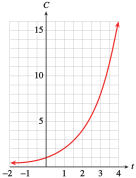
\includegraphics[width=0.4\linewidth]{images/fig-ex-1-2-35}
\leavevmode%
\begin{enumerate}[label=\alph*]
\item\hypertarget{li-117}{}When did \(2000\) students consider themselves computer literate?%
\item\hypertarget{li-118}{}How long did it take that number to double?%
\item\hypertarget{li-119}{}How long did it take for the number to double again?%
\item\hypertarget{li-120}{}How many students became computer literate between January 1992 and June 1993?%
\end{enumerate}
\par\smallskip
\noindent\textbf{Answer.}\hypertarget{answer-28}{}\quad
\leavevmode%
\begin{enumerate}[label=\alph*]
\item\hypertarget{li-121}{}1991%
\item\hypertarget{li-122}{}1 yr%
\item\hypertarget{li-123}{}1 yr%
\item\hypertarget{li-124}{}About 7300%
\end{enumerate}
%
\exercise[36.]\hypertarget{exercise-46}{}The graph shows \(P\) as a function of \(t\). \(P\) is the number of people in Cedar Grove who owned a portable DVD player \(t\) years after 2000.%
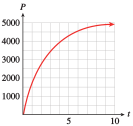
\includegraphics[width=0.4\linewidth]{images/fig-ex-1-2-36}
\leavevmode%
\begin{enumerate}[label=\alph*]
\item\hypertarget{li-125}{}When did 3500 people own portable DVD players?%
\item\hypertarget{li-126}{}How many people owned portable DVD players in 2005?%
\item\hypertarget{li-127}{}The number of owners of portable DVD players in Cedar Grove seems to be leveling off at what number?%
\item\hypertarget{li-128}{}How many people acquired portable DVD players between 2001 and 2004?%
\end{enumerate}
\exercise[37.]\hypertarget{exercise-47}{}The graph shows the revenue, \(R\), a movie theater collects as a function of the price, \(d\), it charges for a ticket.%
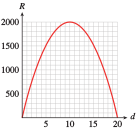
\includegraphics[width=0.5\linewidth]{images/fig-ex-1-2-37}
\leavevmode%
\begin{enumerate}[label=\alph*]
\item\hypertarget{li-129}{}What is the revenue if the theater charges \(\$12.00\) for a ticket?%
\item\hypertarget{li-130}{}What should the theater charge for a ticket in order to collect \(\$1500\) in revenue?%
\item\hypertarget{li-131}{}For what values of \(d\) is \(R\gt 1875\)?%
\end{enumerate}
\par\smallskip
\noindent\textbf{Answer.}\hypertarget{answer-29}{}\quad
\leavevmode%
\begin{enumerate}[label=\alph*]
\item\hypertarget{li-132}{}Approximately \(\$1920\)%
\item\hypertarget{li-133}{}\(\$5\) or \(\$15\)%
\item\hypertarget{li-134}{}\(7.50\lt d\lt 12.50\)%
\end{enumerate}
%
\exercise[38.]\hypertarget{exercise-48}{}The graph shows \(S\) as a function of \(w\). \(S\) represents the weekly sales of a best-selling book, in thousands of dollars, \(w\) weeks after it is released.%
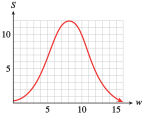
\includegraphics[width=0.5\linewidth]{images/fig-ex-1-2-38}
\leavevmode%
\begin{enumerate}[label=\alph*]
\item\hypertarget{li-135}{}In which weeks were sales over \(\$7000\)?%
\item\hypertarget{li-136}{}In which week did sales fall below \(\$5000\) on their way down?%
\item\hypertarget{li-137}{}For what values of \(w\) is \(S\gt 3.4\)?%
\end{enumerate}
\exercise[39.]\hypertarget{exercise-49}{}The graph shows the federal minimum wage, \(M\), as a function of time, \(t\), adjusted for inflation to reflect its buying power in 2004 dollars. (Source: www.infoplease.com) 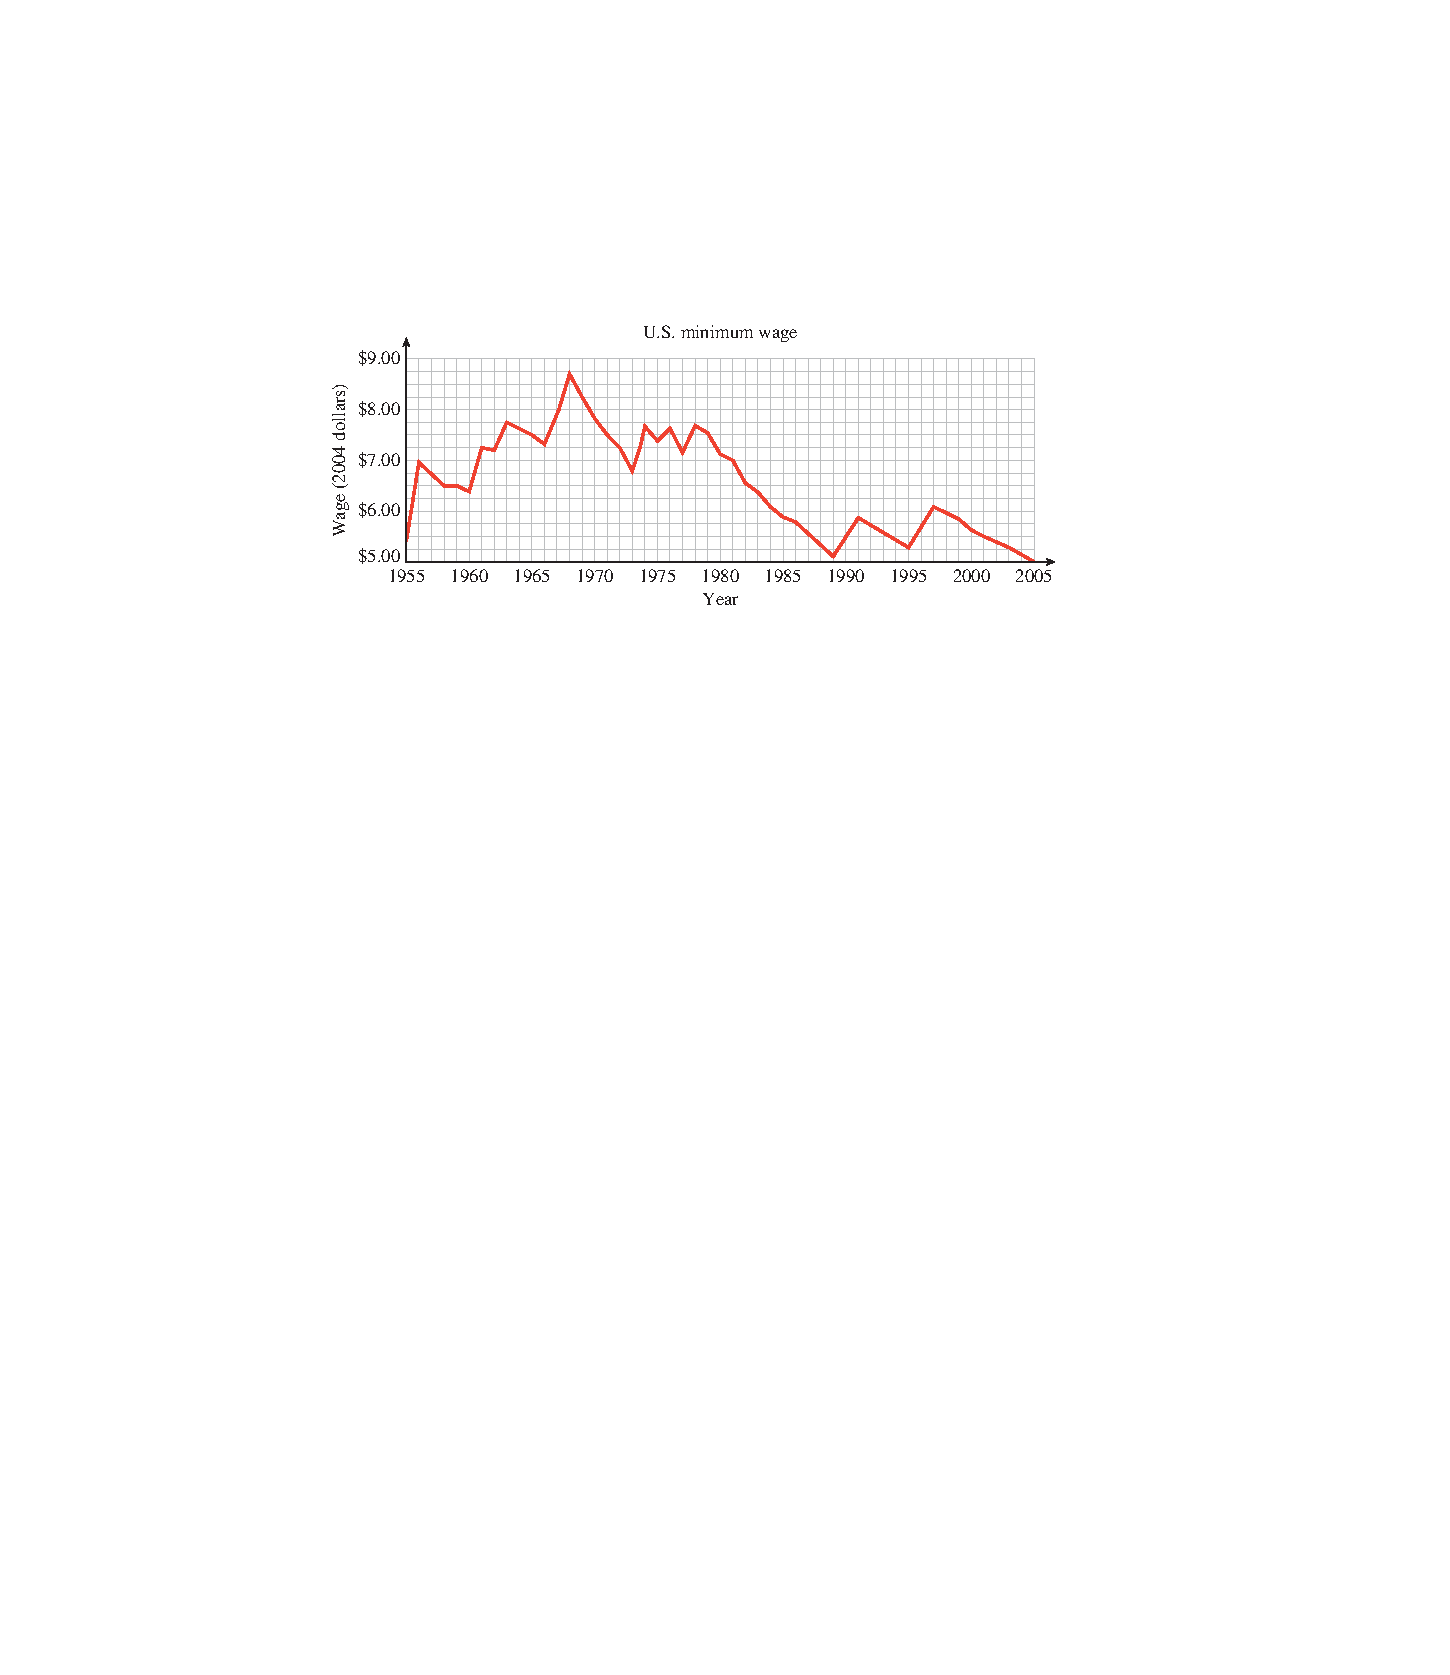
\includegraphics[width=1\linewidth]{images/fig-ex-1-2-39}
 \leavevmode%
\begin{enumerate}[label=\alph*]
\item\hypertarget{li-138}{}When did the minimum wage reach its highest buying power, and what was it worth in 2004 dollars?%
\item\hypertarget{li-139}{}When did the minimum wage fall to its lowest buying power after its peak, and what was its worth at that time?%
\item\hypertarget{li-140}{}Give two years in which the minimum wage was worth \(\$8\) in 2004 dollars.%
\end{enumerate}
%
\par\smallskip
\noindent\textbf{Answer.}\hypertarget{answer-30}{}\quad
\leavevmode%
\begin{enumerate}[label=\alph*]
\item\hypertarget{li-141}{}1968, about \(\$8.70\)%
\item\hypertarget{li-142}{}1989, about \(\$5.10\)%
\item\hypertarget{li-143}{}1967, approximately 1970%
\end{enumerate}
%
\exercise[40.]\hypertarget{exercise-50}{}The graph shows the U.S. unemployment rate, \(U\), as a function of time, \(t\), for the years 1985–2004. (Source: U.S. Bureau of Labor Statistics) 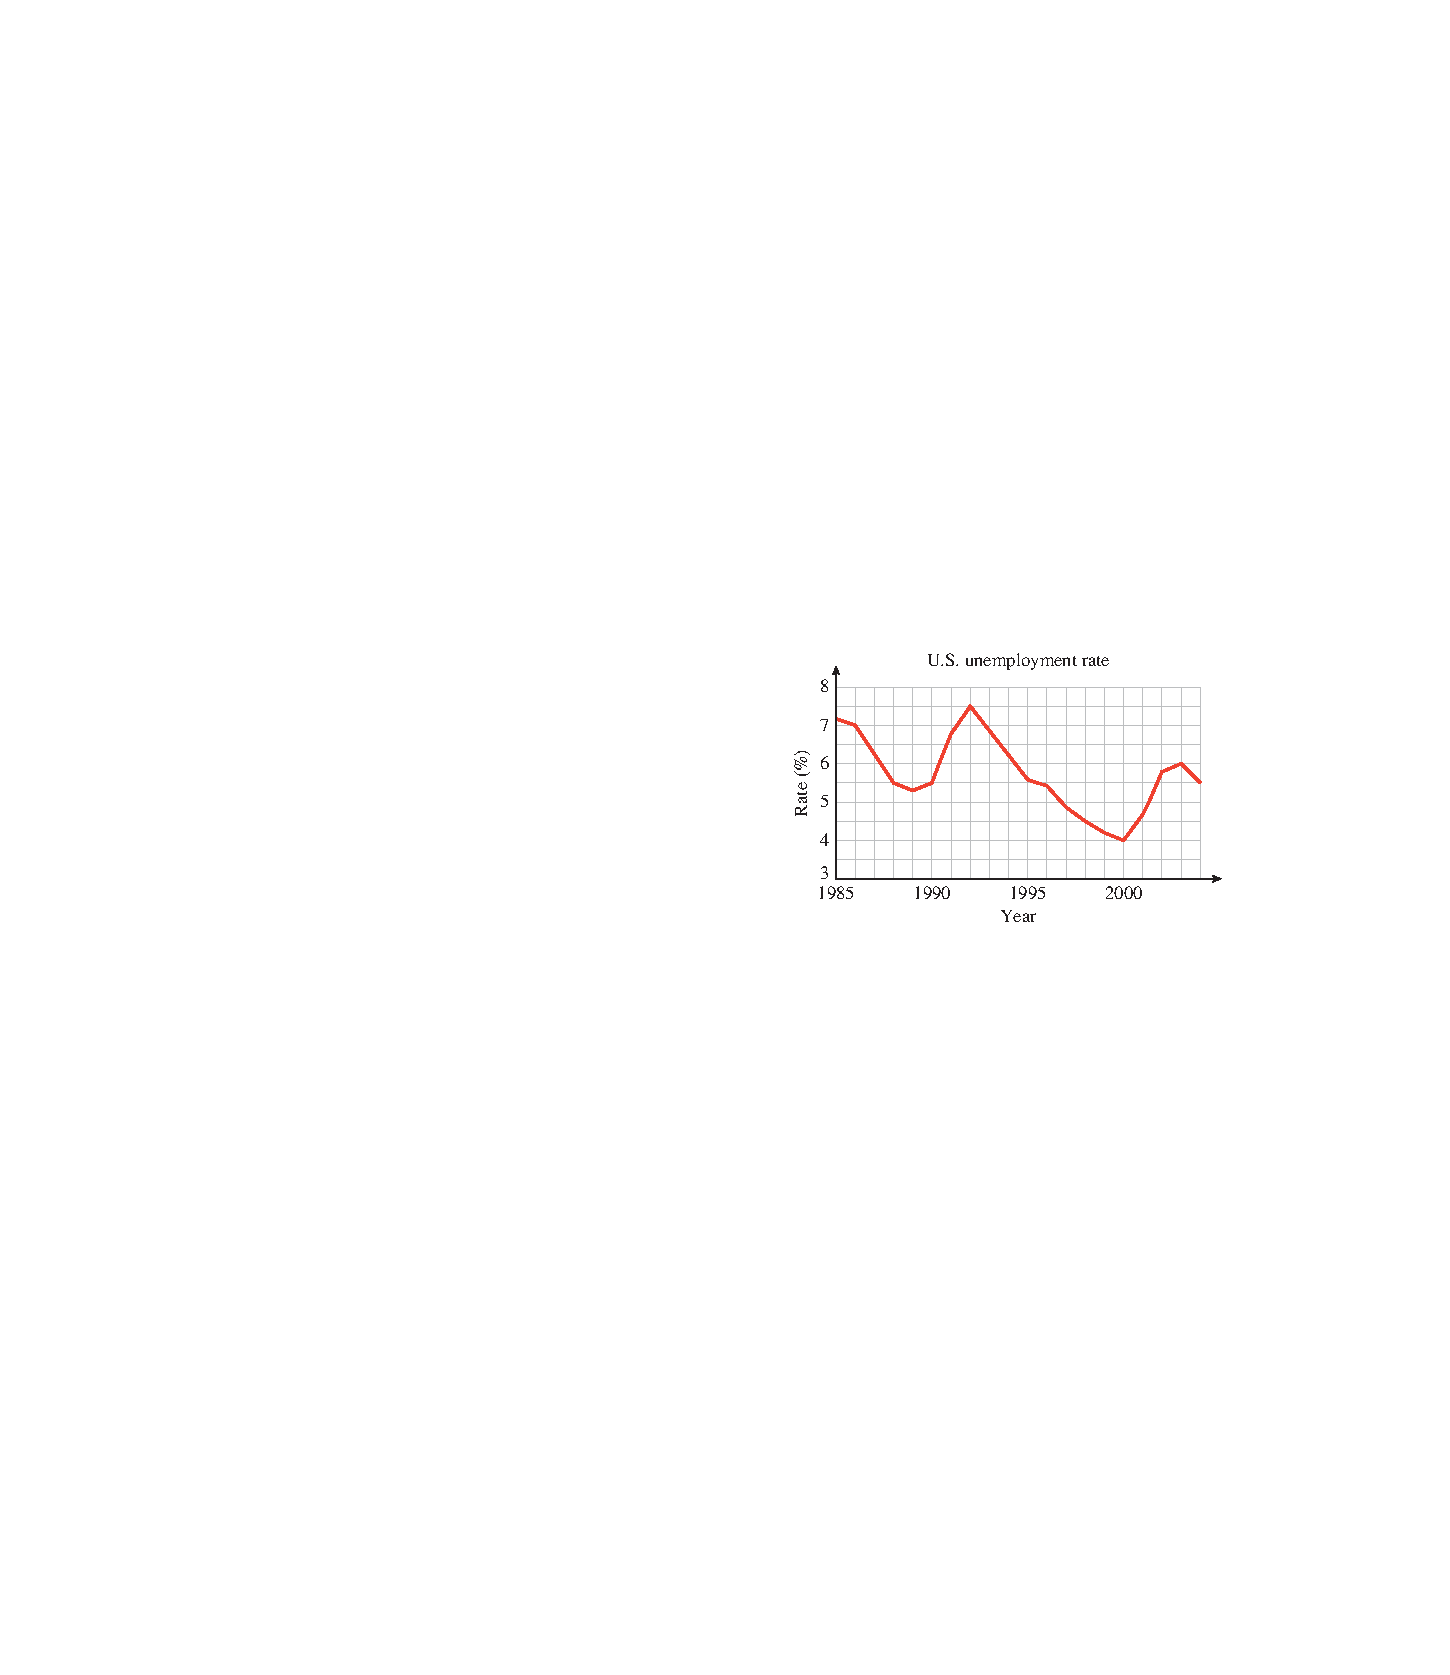
\includegraphics[width=0.6\linewidth]{images/fig-ex-1-2-40}
 \leavevmode%
\begin{enumerate}[label=\alph*]
\item\hypertarget{li-144}{}When did the unemployment rate reach its highest value, and what was its highest value?%
\item\hypertarget{li-145}{}When did the unemployment rate fall to its lowest value, and what was its lowest value?%
\item\hypertarget{li-146}{}Give two years in which the unemployment rate was \(4.5\%\).%
\end{enumerate}
%
\end{exercisegroup}
\par\smallskip\noindent
\hypertarget{exercisegroup-6}{}\par\noindent In Problems 41–48, evaluate each function for the given values.%
\begin{exercisegroup}(2)
\exercise[41.]\hypertarget{exercise-51}{}\(f (x) = 6 - 2x\) \leavevmode%
\begin{multicols}{2}
\begin{enumerate}[label=\alph*]
\item\hypertarget{li-147}{}\(f(3)\)%
\item\hypertarget{li-148}{}\(f(-2)\)%
\item\hypertarget{li-149}{}\(f(12.7)\)%
\item\hypertarget{li-150}{}\(f\left(\dfrac{2}{3}\right)\)%
\end{enumerate}
\end{multicols}
%
\par\smallskip
\noindent\textbf{Answer.}\hypertarget{answer-31}{}\quad
\leavevmode%
\begin{multicols}{2}
\begin{enumerate}[label=\alph*]
\item\hypertarget{li-151}{}\(0\)%
\item\hypertarget{li-152}{}\(10\)%
\item\hypertarget{li-153}{}\(-19.4\)%
\item\hypertarget{li-154}{}\(\dfrac{14}{3} \)%
\end{enumerate}
\end{multicols}
%
\exercise[42.]\hypertarget{exercise-52}{}\(g(t) = 5t - 3\) \leavevmode%
\begin{multicols}{2}
\begin{enumerate}[label=\alph*]
\item\hypertarget{li-155}{}\(g(1)\)%
\item\hypertarget{li-156}{}\(g(-4)\)%
\item\hypertarget{li-157}{}\(g(14.1)\)%
\item\hypertarget{li-158}{}\(g\left(\dfrac{3}{4}\right)\)%
\end{enumerate}
\end{multicols}
%
\exercise[43.]\hypertarget{exercise-53}{}\(h(v) = 2v^2 - 3v + 1\) \leavevmode%
\begin{multicols}{2}
\begin{enumerate}[label=\alph*]
\item\hypertarget{li-159}{}\(h(0)\)%
\item\hypertarget{li-160}{}\(h(-1)\)%
\item\hypertarget{li-161}{}\(h\left(\dfrac{1}{4}\right)\)%
\item\hypertarget{li-162}{}\(h(-6.2)\)%
\end{enumerate}
\end{multicols}
%
\par\smallskip
\noindent\textbf{Answer.}\hypertarget{answer-32}{}\quad
\leavevmode%
\begin{multicols}{2}
\begin{enumerate}[label=\alph*]
\item\hypertarget{li-163}{}\(1\)%
\item\hypertarget{li-164}{}\(6\)%
\item\hypertarget{li-165}{}\(\dfrac{3}{8}\)%
\item\hypertarget{li-166}{}\(96.48 \)%
\end{enumerate}
\end{multicols}
%
\exercise[44.]\hypertarget{exercise-54}{}\(r (s) = 2s - s^2\) \leavevmode%
\begin{multicols}{2}
\begin{enumerate}[label=\alph*]
\item\hypertarget{li-167}{}\(r(2)\)%
\item\hypertarget{li-168}{}\(r(-4)\)%
\item\hypertarget{li-169}{}\(r\left(\dfrac{1}{3}\right)\)%
\item\hypertarget{li-170}{}\(r(-1.3)\)%
\end{enumerate}
\end{multicols}
%
\exercise[45.]\hypertarget{exercise-55}{}\(H(z) = \dfrac{2z - 3}{z + 2}\) \leavevmode%
\begin{multicols}{2}
\begin{enumerate}[label=\alph*]
\item\hypertarget{li-171}{}\(H(4)\)%
\item\hypertarget{li-172}{}\(H(-3)\)%
\item\hypertarget{li-173}{}\(H\left(\dfrac{4}{3}\right)\)%
\item\hypertarget{li-174}{}\(H(4.5)\)%
\end{enumerate}
\end{multicols}
%
\par\smallskip
\noindent\textbf{Answer.}\hypertarget{answer-33}{}\quad
\leavevmode%
\begin{multicols}{2}
\begin{enumerate}[label=\alph*]
\item\hypertarget{li-175}{}\(\dfrac{5}{6} \)%
\item\hypertarget{li-176}{}\(9\)%
\item\hypertarget{li-177}{}\(\dfrac{-1}{10}\)%
\item\hypertarget{li-178}{}\(\dfrac{12}{13}\approx 0.923 \)%
\end{enumerate}
\end{multicols}
%
\exercise[46.]\hypertarget{exercise-56}{}\(F(x) = \dfrac{1-x}{2x-3}\) \leavevmode%
\begin{multicols}{2}
\begin{enumerate}[label=\alph*]
\item\hypertarget{li-179}{}\(F(0)\)%
\item\hypertarget{li-180}{}\(F(-3)\)%
\item\hypertarget{li-181}{}\(F\left(\dfrac{5}{2}\right)\)%
\item\hypertarget{li-182}{}\(F(9.8)\)%
\end{enumerate}
\end{multicols}
%
\exercise[47.]\hypertarget{exercise-57}{}\(E(t) =\sqrt{t-4}\) \leavevmode%
\begin{multicols}{2}
\begin{enumerate}[label=\alph*]
\item\hypertarget{li-183}{}\(E(16)\)%
\item\hypertarget{li-184}{}\(E(4)\)%
\item\hypertarget{li-185}{}\(E(7)\)%
\item\hypertarget{li-186}{}\(E(4.2)\)%
\end{enumerate}
\end{multicols}
%
\par\smallskip
\noindent\textbf{Answer.}\hypertarget{answer-34}{}\quad
\leavevmode%
\begin{multicols}{2}
\begin{enumerate}[label=\alph*]
\item\hypertarget{li-187}{}\(\sqrt{12} \)%
\item\hypertarget{li-188}{}\(0\)%
\item\hypertarget{li-189}{}\(\sqrt{3}\)%
\item\hypertarget{li-190}{}\(\sqrt{0.2}\approx 0.447 \)%
\end{enumerate}
\end{multicols}
%
\exercise[48.]\hypertarget{exercise-58}{}\(D(r) =\sqrt{5-r}\) \leavevmode%
\begin{multicols}{2}
\begin{enumerate}[label=\alph*]
\item\hypertarget{li-191}{}\(D(4)\)%
\item\hypertarget{li-192}{}\(D(-3)\)%
\item\hypertarget{li-193}{}\(D(-9)\)%
\item\hypertarget{li-194}{}\(D(4.6)\)%
\end{enumerate}
\end{multicols}
%
\end{exercisegroup}
\par\smallskip\noindent
\item[49.]\hypertarget{exercise-59}{}A sport utility vehicle costs \(\$28,000\) and depreciates according to the formula \(V(t) = 28,000 (1 - 0.08t)\),where \(V\) is the value of the vehicle after \(t\) years. \leavevmode%
\begin{enumerate}[label=\alph*]
\item\hypertarget{li-195}{}Evaluate \(V(12)\) and explain what it means.%
\item\hypertarget{li-196}{}Solve the equation \(V(t) = 0\) and explain what it means.%
\item\hypertarget{li-197}{}If this year is \(t = n\), what does \(V(n + 2)\) mean?%
\end{enumerate}
%
\par\smallskip
\par\smallskip
\noindent\textbf{Answer.}\hypertarget{answer-35}{}\quad
\leavevmode%
\begin{enumerate}[label=\alph*]
\item\hypertarget{li-198}{}\(V(12) = 1120\): After 12 years, the SUV is worth \(\$1120\).%
\item\hypertarget{li-199}{}\(t = 12.5\): The SUV has zero value after \(12\frac{1}{2}\) years.%
\item\hypertarget{li-200}{}The value 2 years later%
\end{enumerate}
%
\item[50.]\hypertarget{exercise-60}{}In a profit-sharing plan, an employee receives a salary of \(S(x) = 20,000 + 0.01x\), where \(x\) represents the company's profit for the year. \leavevmode%
\begin{enumerate}[label=\alph*]
\item\hypertarget{li-201}{}Evaluate \(S(850,000)\) and explain what it means.%
\item\hypertarget{li-202}{}Solve the equation \(S(x) = 30,000\) and explain what it means.%
\item\hypertarget{li-203}{}If the company made a profit of \(p\) dollars this year, what does \(S(2p)\) mean?%
\end{enumerate}
%
\par\smallskip
\item[51.]\hypertarget{exercise-61}{}The number of compact cars that a large dealership can sell at price \(p\) is given by \(N( p) = \dfrac{12,000,000}{p}\). \leavevmode%
\begin{enumerate}[label=\alph*]
\item\hypertarget{li-204}{}Evaluate \(N(6000)\) and explain what it means.%
\item\hypertarget{li-205}{}As \(p\) increases, does \(N(p)\) increase or decrease? Why is this reasonable?%
\item\hypertarget{li-206}{}If the current price for a compact car is \(D\), what does \(2N(D)\) mean?%
\end{enumerate}
%
\par\smallskip
\par\smallskip
\noindent\textbf{Answer.}\hypertarget{answer-36}{}\quad
\leavevmode%
\begin{enumerate}[label=\alph*]
\item\hypertarget{li-207}{}\(N(6000) = 2000\): \(2000\) cars will be sold at a price of \(\$6000\).%
\item\hypertarget{li-208}{}\(N(p)\) decreases with increasing \(p\) because fewer cars will be sold when the price increases.%
\item\hypertarget{li-209}{}\(2N(D)\) represents twice the number of cars that can be sold at the current price.%
\end{enumerate}
%
\item[52.]\hypertarget{exercise-62}{}A department store finds that the market value of its Christmas-related merchandise is given by \(M(t) = \dfrac{600,000}{t},~ t\le 30\), where \(t\) is the number of weeks after Christmas. \leavevmode%
\begin{enumerate}[label=\alph*]
\item\hypertarget{li-210}{}Evaluate \(M(2)\) and explain what it means.%
\item\hypertarget{li-211}{}As \(t\) increases, does \(M(t)\) increase or decrease? Why is this reasonable?%
\item\hypertarget{li-212}{}If this week \(t = n\), what does \(M(n + 1)\) mean?%
\end{enumerate}
%
\par\smallskip
\item[53.]\hypertarget{exercise-63}{}The velocity of a car that brakes suddenly can be determined from the length of its skid marks, \(d\), by \(v(d) = \sqrt{12d}\), where \(d\) is in feet and \(v\) is in miles per hour. \leavevmode%
\begin{enumerate}[label=\alph*]
\item\hypertarget{li-213}{}Evaluate \(v(250)\) and explain what it means.%
\item\hypertarget{li-214}{}Estimate the length of the skid marks left by a car traveling at \(100\) miles per hour.%
\item\hypertarget{li-215}{}Write your answer to part (b) with function notation.%
\end{enumerate}
%
\par\smallskip
\par\smallskip
\noindent\textbf{Answer.}\hypertarget{answer-37}{}\quad
\leavevmode%
\begin{enumerate}[label=\alph*]
\item\hypertarget{li-216}{}\(v(250) = 54.8\) is the speed of a car that left \(250\)-foot skid marks.%
\item\hypertarget{li-217}{}\(833\dfrac{1}{3}\) feet%
\item\hypertarget{li-218}{}\(v\left(833\dfrac{1}{3}\right)= 100\)%
\end{enumerate}
%
\item[54.]\hypertarget{exercise-64}{}The distance, \(d\), in miles that a person can see on a clear day from a height, \(h\), in feet is given by \(d(h) = 1.22\sqrt{h}\). \leavevmode%
\begin{enumerate}[label=\alph*]
\item\hypertarget{li-219}{}Evaluate \(d(20,320)\) and explain what it means.%
\item\hypertarget{li-220}{}Estimate the height you need in order to see \(100\) miles.%
\item\hypertarget{li-221}{}Write your answer to part (b) with function notation.%
\end{enumerate}
%
\par\smallskip
\item[55.]\hypertarget{exercise-65}{}The figure gives data about snowfall, air temperature, and number of avalanches on the Mikka glacier in Sarek, Lapland, in 1957. (Source: Leopold, Wolman, Miller, 1992) 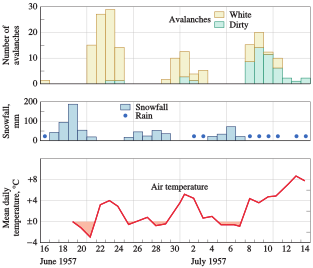
\includegraphics[width=1\linewidth]{images/fig-ex-1-2-55}
 \leavevmode%
\begin{enumerate}[label=\alph*]
\item\hypertarget{li-222}{}During June and July, avalanches occurred over three separate time intervals. What were they?%
\item\hypertarget{li-223}{}Over what three time intervals did snow fall?%
\item\hypertarget{li-224}{}When was the temperature above freezing (\(0\degree\)C)?%
\item\hypertarget{li-225}{}Using your answers to parts (a)–(c), make a conjecture about the conditions that encourage avalanches.%
\end{enumerate}
%
\par\smallskip
\par\smallskip
\noindent\textbf{Answer.}\hypertarget{answer-38}{}\quad
\leavevmode%
\begin{enumerate}[label=\alph*]
\item\hypertarget{li-226}{}June 21–24, June 29–July 3, July 8–14%
\item\hypertarget{li-227}{}June 17–21, June 25–29, July 4–7%
\item\hypertarget{li-228}{}June 22–24, June 27, June 29–July 4, July 8–14%
\item\hypertarget{li-229}{}Avalanches occur when temperatures rise above freezing immediately after snowfall.%
\end{enumerate}
%
\item[56.]\hypertarget{exercise-66}{}The bar graph shows the percent of Earth's surface that lies at various altitudes or depths below the surface of the oceans. (Depths are given as negative altitudes.) (Source: Open University) 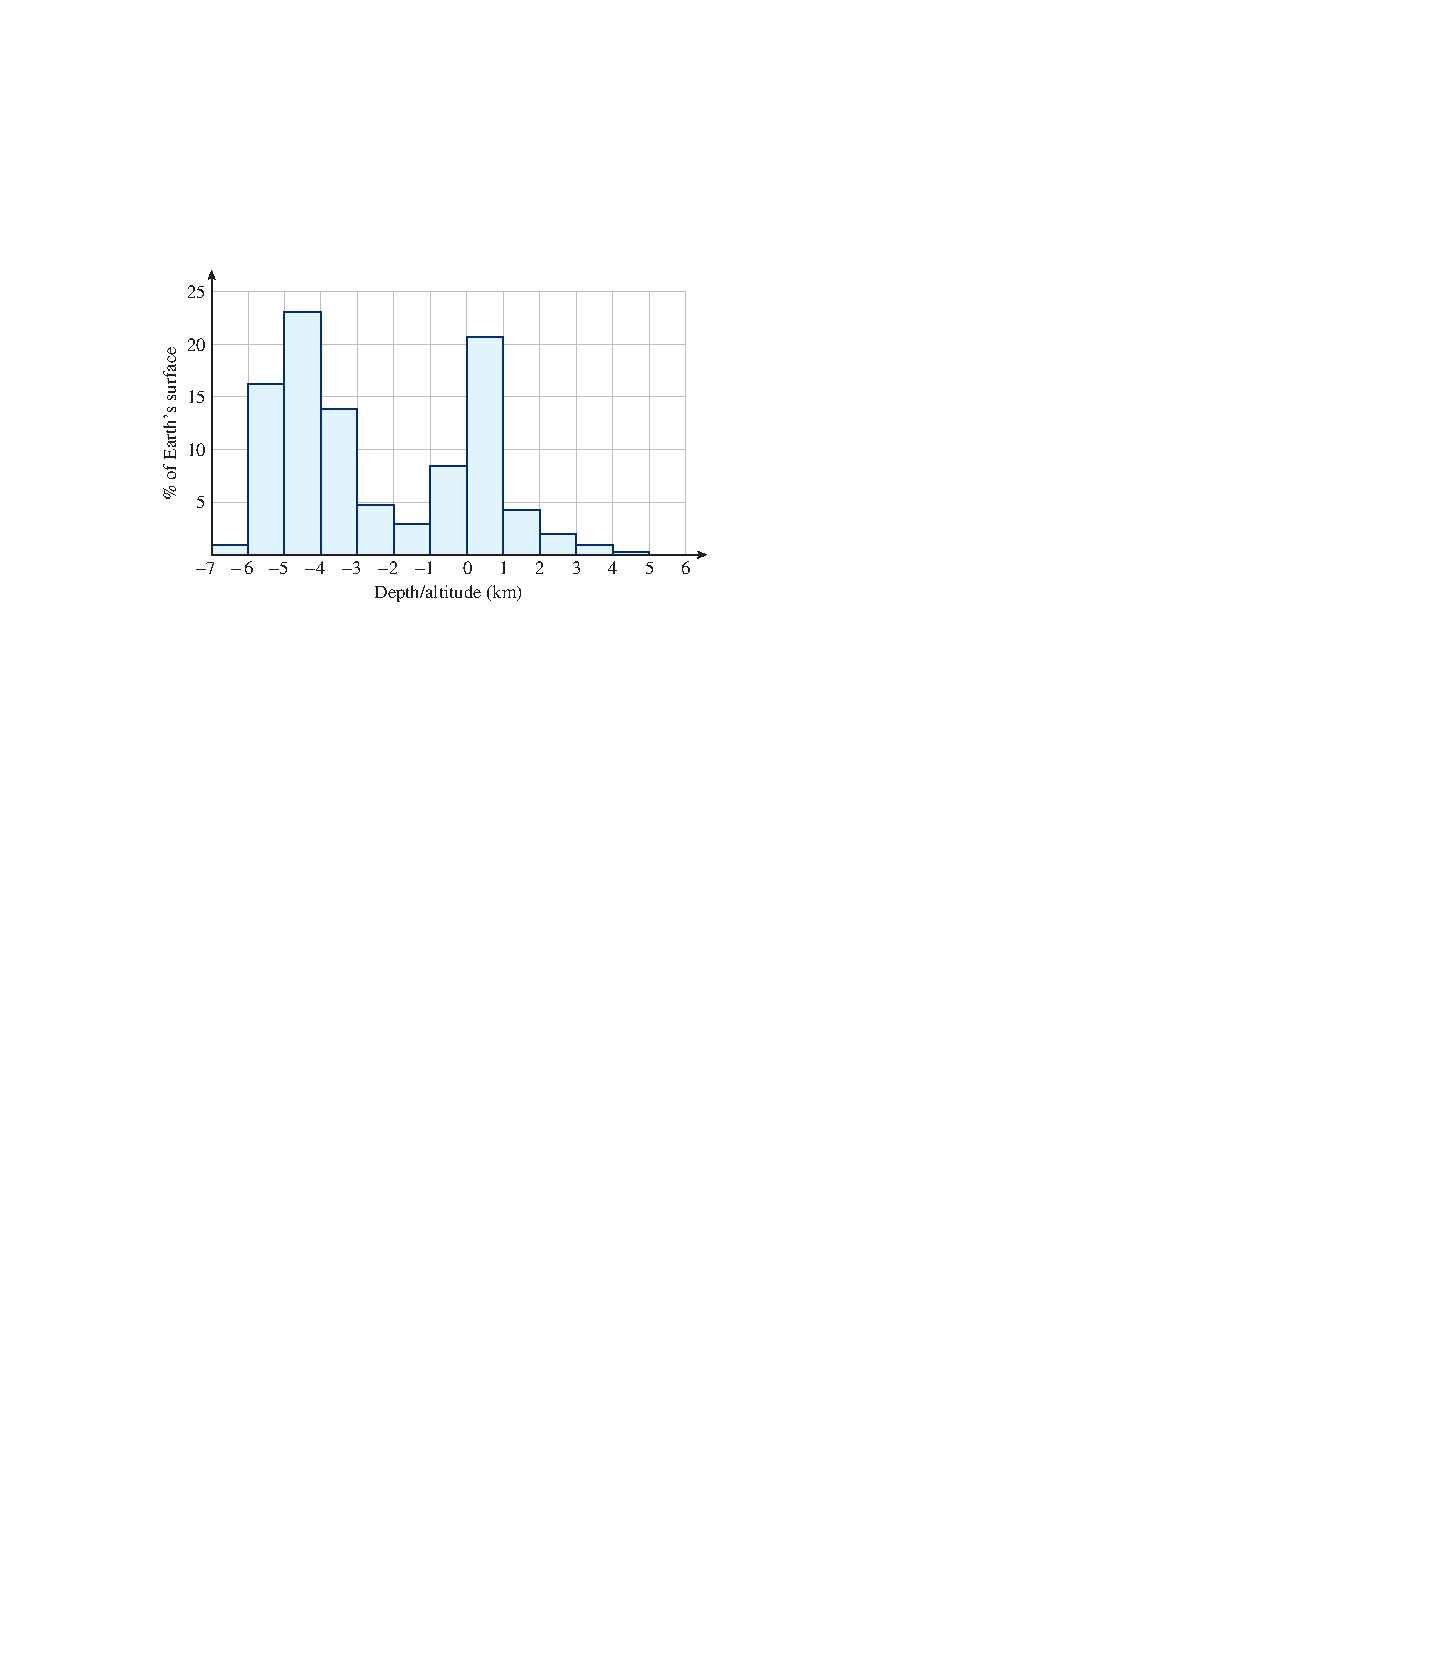
\includegraphics[width=0.7\linewidth]{images/fig-ex-1-2-56}
 \leavevmode%
\begin{enumerate}[label=\alph*]
\item\hypertarget{li-230}{}Read the graph and complete the table. \begin{tabular}{AcAcA}\hrulethick
Altitude (km)&\tablecelllines{c}{m}
{Percent of\\
Earth's surface}
\tabularnewline\hrulethin
\(-7\) to \(-6\)&\(\)\tabularnewline\hrulethin
\(-6\) to \(-5\)&\(\)\tabularnewline\hrulethin
\(-5\) to \(-4\)&\(\)\tabularnewline\hrulethin
\(-4\) to \(-3\)&\(\)\tabularnewline\hrulethin
\(-3\) to \(-2\)&\(\)\tabularnewline\hrulethin
\(-2\) to \(-1\)&\(\)\tabularnewline\hrulethin
\(-1\) to \(0\)&\(\)\tabularnewline\hrulethin
\(0\) to \(1\)&\(\)\tabularnewline\hrulethin
\(1\) to \(2\)&\(\)\tabularnewline\hrulethin
\(2\) to \(3\)&\(\)\tabularnewline\hrulethin
\(3\) to \(4\)&\(\)\tabularnewline\hrulethin
\(4\) to \(5\)&\(\)\tabularnewline\hrulethin
\end{tabular}
%
\item\hypertarget{li-231}{}What is the most common altitude? What is the second most common altitude??%
\item\hypertarget{li-232}{}Approximately what percent of the Earth's surface is below sea level?%
\item\hypertarget{li-233}{}The height of Mt. Everest is \(8.85\) kilometers. Can you think of a reason why it is not included in the graph?%
\end{enumerate}
%
\par\smallskip
\item[57.]\hypertarget{exercise-67}{}The graph shows the temperature of the ocean at various depths. (Source: Open University) 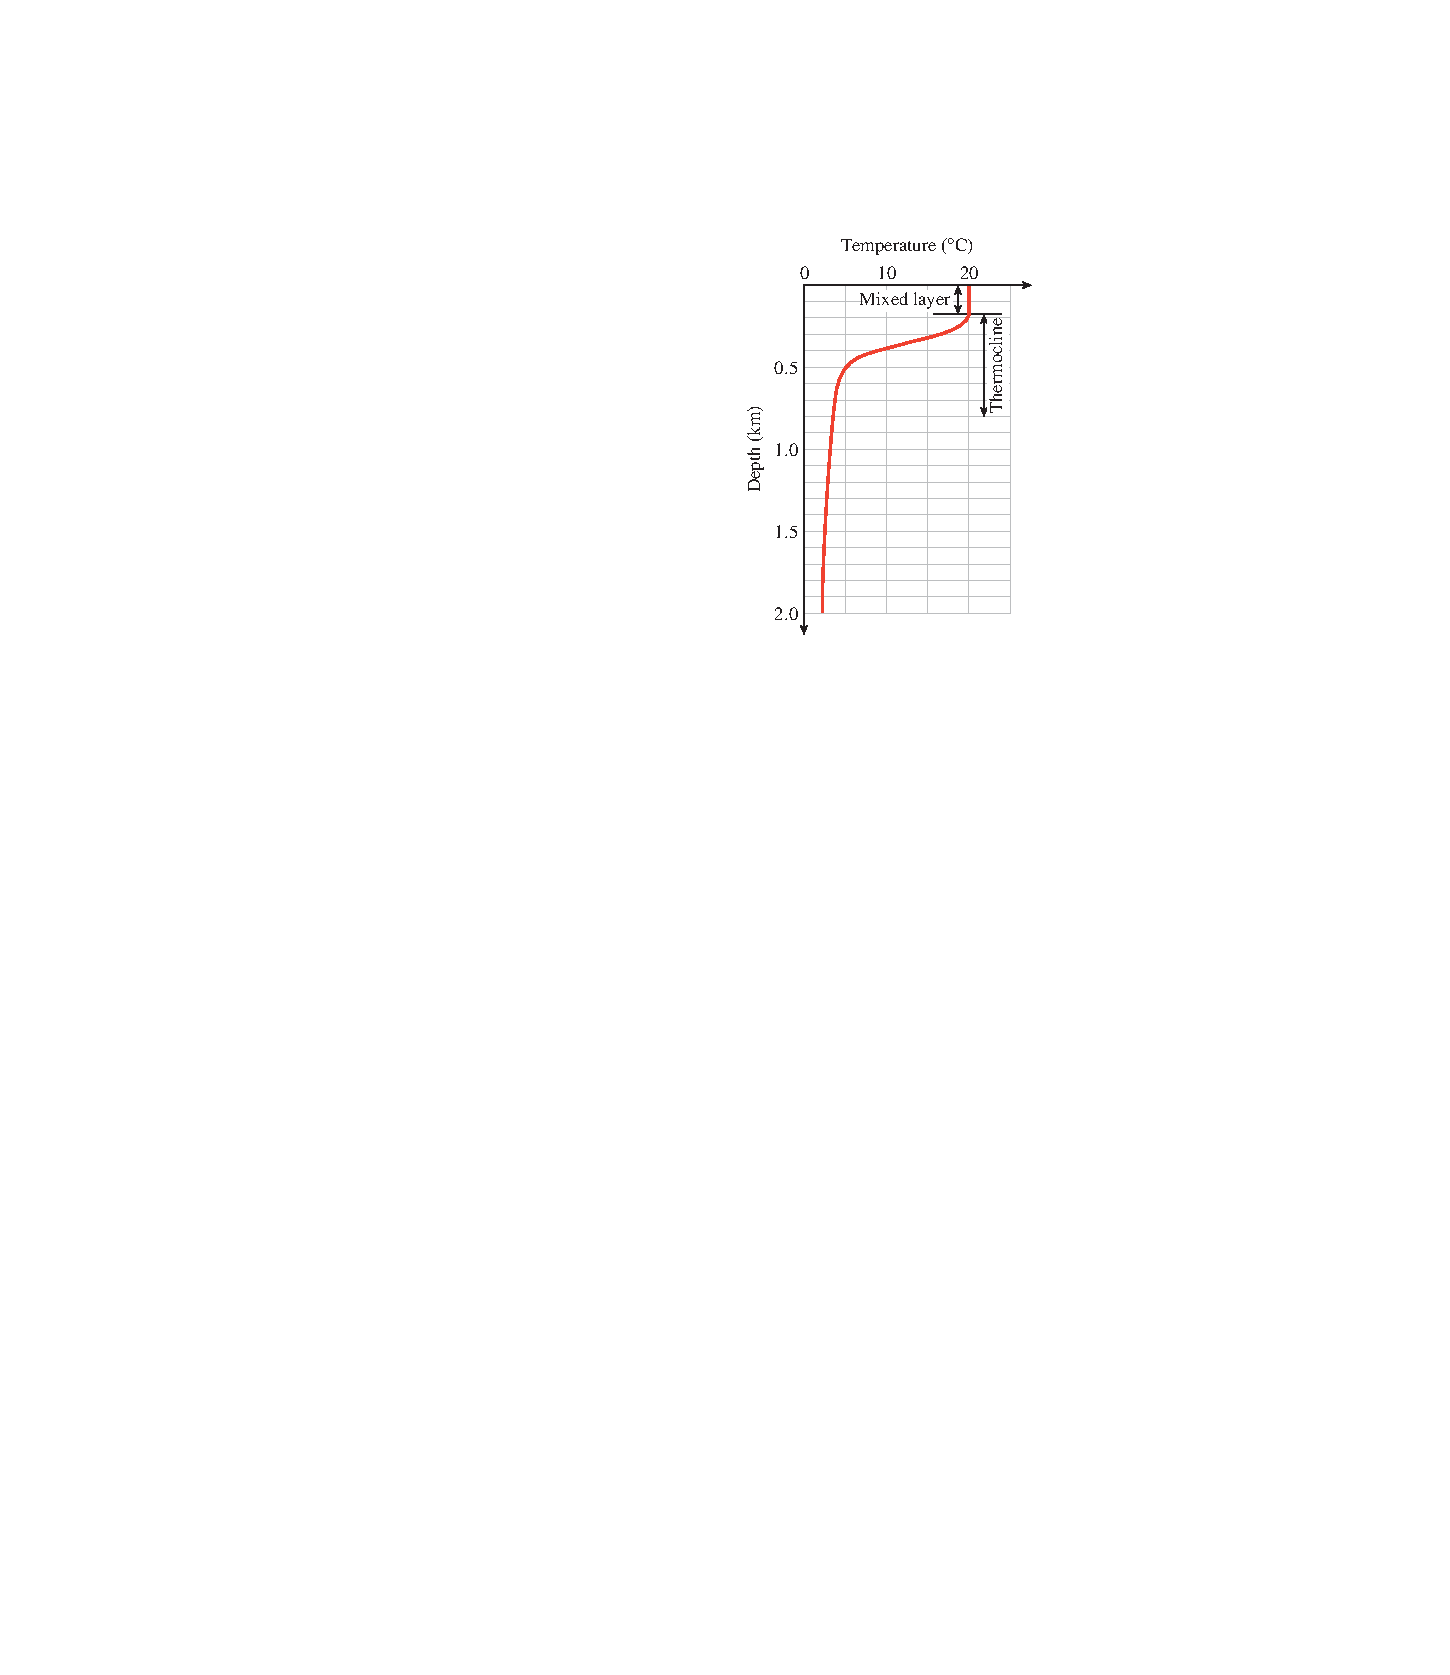
\includegraphics[width=0.4\linewidth]{images/fig-ex-1-2-57}
 \leavevmode%
\begin{enumerate}[label=\alph*]
\item\hypertarget{li-234}{}Is depth a function of temperature?%
\item\hypertarget{li-235}{}Is temperature a function of depth?%
\item\hypertarget{li-236}{}The axes are scaled in an unusual way. Why is it useful to present the graph in this way?%
\end{enumerate}
%
\par\smallskip
\par\smallskip
\noindent\textbf{Answer.}\hypertarget{answer-39}{}\quad
\leavevmode%
\begin{enumerate}[label=\alph*]
\item\hypertarget{li-237}{}No%
\item\hypertarget{li-238}{}Yes%
\item\hypertarget{li-239}{}Moving downwards on the graph corresponds to moving downwards in the ocean.%
\end{enumerate}
%
\item[58.]\hypertarget{exercise-68}{}The graph shows the relationship between annual precipitation, \(p\), in a region and the amount of erosion, measured in tons per square mile, \(s\). (Source: Leopold, Wolman, Miller, 1992) 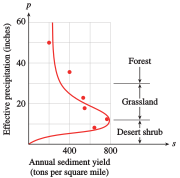
\includegraphics[width=0.5\linewidth]{images/fig-ex-1-2-58}
 \leavevmode%
\begin{enumerate}[label=\alph*]
\item\hypertarget{li-240}{}Is the amount of erosion a function of the amount of precipitation?%
\item\hypertarget{li-241}{}At what annual precipitation is erosion at a maximum, and what is that maximum?%
\item\hypertarget{li-242}{}Over what interval of annual precipitation does erosion decrease?%
\item\hypertarget{li-243}{}An increase in vegetation inhibits erosion, and precipitation encourages vegetation. What happens to the amount of erosion as precipitation increases in each of these three environments? \begin{tabular}{ll}
desert shrub&\(0\lt 0\lt 12\)\tabularnewline[0pt]
grassland&\(12\lt 0\lt 30\)\tabularnewline[0pt]
forest&\(30\lt 0\lt 60\)
\end{tabular}
%
\end{enumerate}
%
\par\smallskip
\hypertarget{exercisegroup-7}{}\par\noindent Evaluate the function and simplify.%
\begin{exercisegroup}(2)
\exercise[59.]\hypertarget{exercise-69}{}\(G(s) = 3s^2 - 6s\) \leavevmode%
\begin{multicols}{2}
\begin{enumerate}[label=\alph*]
\item\hypertarget{li-244}{}\(G(3a)\)%
\item\hypertarget{li-245}{}\(G(a + 2)\)%
\item\hypertarget{li-246}{}\(G(a) + 2\)%
\item\hypertarget{li-247}{}\(G(-a)\)%
\end{enumerate}
\end{multicols}
%
\par\smallskip
\noindent\textbf{Answer.}\hypertarget{answer-40}{}\quad
\leavevmode%
\begin{multicols}{2}
\begin{enumerate}[label=\alph*]
\item\hypertarget{li-248}{}\(27a^2 - 18a\)%
\item\hypertarget{li-249}{}\(3a^2 + 6a\)%
\item\hypertarget{li-250}{}\(3a^2 - 6a + 2\)%
\item\hypertarget{li-251}{}\(3a^2 + 6a \)%
\end{enumerate}
\end{multicols}
%
\exercise[60.]\hypertarget{exercise-70}{}\(h(x) = 2x^2 + 6x - 3\) \leavevmode%
\begin{multicols}{2}
\begin{enumerate}[label=\alph*]
\item\hypertarget{li-252}{}\(h(2a)\)%
\item\hypertarget{li-253}{}\(h(a + 3)\)%
\item\hypertarget{li-254}{}\(h(a) + 3\)%
\item\hypertarget{li-255}{}\(h(-a)\)%
\end{enumerate}
\end{multicols}
%
\exercise[61.]\hypertarget{exercise-71}{}\(g(x) = 8\) \leavevmode%
\begin{multicols}{2}
\begin{enumerate}[label=\alph*]
\item\hypertarget{li-256}{}\(g(2)\)%
\item\hypertarget{li-257}{}\(g(8)\)%
\item\hypertarget{li-258}{}\(g(a + 1)\)%
\item\hypertarget{li-259}{}\(g(-x)\)%
\end{enumerate}
\end{multicols}
%
\par\smallskip
\noindent\textbf{Answer.}\hypertarget{answer-41}{}\quad
\leavevmode%
\begin{multicols}{2}
\begin{enumerate}[label=\alph*]
\item\hypertarget{li-260}{}\(8\)%
\item\hypertarget{li-261}{}\(8\)%
\item\hypertarget{li-262}{}\(8\)%
\item\hypertarget{li-263}{}\(8 \)%
\end{enumerate}
\end{multicols}
%
\exercise[62.]\hypertarget{exercise-72}{}\(f (t) = -3\) \leavevmode%
\begin{multicols}{2}
\begin{enumerate}[label=\alph*]
\item\hypertarget{li-264}{}\(f (4)\)%
\item\hypertarget{li-265}{}\(f (-3)\)%
\item\hypertarget{li-266}{}\(f (b - 2)\)%
\item\hypertarget{li-267}{}\(f (-t)\)%
\end{enumerate}
\end{multicols}
%
\exercise[63.]\hypertarget{exercise-73}{}\(P(x) = x^3 - 1\) \leavevmode%
\begin{multicols}{2}
\begin{enumerate}[label=\alph*]
\item\hypertarget{li-268}{}\(P(2x)\)%
\item\hypertarget{li-269}{}\(2P(x)\)%
\item\hypertarget{li-270}{}\(P(x^2)\)%
\item\hypertarget{li-271}{}\([P(x)]^2\)%
\end{enumerate}
\end{multicols}
%
\par\smallskip
\noindent\textbf{Answer.}\hypertarget{answer-42}{}\quad
\leavevmode%
\begin{multicols}{2}
\begin{enumerate}[label=\alph*]
\item\hypertarget{li-272}{}\(8x^3 - 1\)%
\item\hypertarget{li-273}{}\(2x^3 - 2\)%
\item\hypertarget{li-274}{}\(x^6 - 1\)%
\item\hypertarget{li-275}{}\(x^6 - 2x^3 + 1 \)%
\end{enumerate}
\end{multicols}
%
\exercise[64.]\hypertarget{exercise-74}{}\(Q(t) = 5t^3\) \leavevmode%
\begin{multicols}{2}
\begin{enumerate}[label=\alph*]
\item\hypertarget{li-276}{}\(Q(2t)\)%
\item\hypertarget{li-277}{}\(2Q(t)\)%
\item\hypertarget{li-278}{}\(Q(t^2)\)%
\item\hypertarget{li-279}{}\([Q(t)]^2\)%
\end{enumerate}
\end{multicols}
%
\end{exercisegroup}
\par\smallskip\noindent
\hypertarget{exercisegroup-8}{}\par\noindent Evaluate each function for the given expressions and simplify.%
\begin{exercisegroup}(2)
\exercise[65.]\hypertarget{exercise-75}{}\(f (x) = x^3\) \leavevmode%
\begin{multicols}{2}
\begin{enumerate}[label=\alph*]
\item\hypertarget{li-280}{}\(f (a^2)\)%
\item\hypertarget{li-281}{}\(a^3 \cdot f (a^3)\)%
\item\hypertarget{li-282}{}\(f (ab)\)%
\item\hypertarget{li-283}{}\(f (a + b)\)%
\end{enumerate}
\end{multicols}
%
\par\smallskip
\noindent\textbf{Answer.}\hypertarget{answer-43}{}\quad
\leavevmode%
\begin{multicols}{2}
\begin{enumerate}[label=\alph*]
\item\hypertarget{li-284}{}\(a^6\)%
\item\hypertarget{li-285}{}\(a^{12}\)%
\item\hypertarget{li-286}{}\(a^3b^3\)%
\item\hypertarget{li-287}{}\(a^3 + 3a^2b + 3ab^2 + b^3 \)%
\end{enumerate}
\end{multicols}
%
\exercise[66.]\hypertarget{exercise-76}{}\(g(x) = x^4\) \leavevmode%
\begin{multicols}{2}
\begin{enumerate}[label=\alph*]
\item\hypertarget{li-288}{}\(g(a^3)\)%
\item\hypertarget{li-289}{}\(a^4\cdot g(a^4)\)%
\item\hypertarget{li-290}{}\(g(ab)\)%
\item\hypertarget{li-291}{}\(g(a + b)\)%
\end{enumerate}
\end{multicols}
%
\exercise[67.]\hypertarget{exercise-77}{}\(F(x) = 3x^5\) \leavevmode%
\begin{multicols}{2}
\begin{enumerate}[label=\alph*]
\item\hypertarget{li-292}{}\(F(2a)\)%
\item\hypertarget{li-293}{}\(2 F(a)\)%
\item\hypertarget{li-294}{}\(F(a^2)\)%
\item\hypertarget{li-295}{}\([F(a)]^2\)%
\end{enumerate}
\end{multicols}
%
\par\smallskip
\noindent\textbf{Answer.}\hypertarget{answer-44}{}\quad
\leavevmode%
\begin{multicols}{2}
\begin{enumerate}[label=\alph*]
\item\hypertarget{li-296}{}\(96a^5\)%
\item\hypertarget{li-297}{}\(6a^5\)%
\item\hypertarget{li-298}{}\(3a^{10}\)%
\item\hypertarget{li-299}{}\(9a^{10} \)%
\end{enumerate}
\end{multicols}
%
\exercise[68.]\hypertarget{exercise-78}{}\(G(x) = 4x^3\) \leavevmode%
\begin{multicols}{2}
\begin{enumerate}[label=\alph*]
\item\hypertarget{li-300}{}\(G(3a)\)%
\item\hypertarget{li-301}{}\(3G(a)\)%
\item\hypertarget{li-302}{}\(G(a^4)\)%
\item\hypertarget{li-303}{}\([G(a)]^4\)%
\end{enumerate}
\end{multicols}
%
\end{exercisegroup}
\par\smallskip\noindent
\hypertarget{exercisegroup-9}{}\par\noindent For the functions in Problems 69–76, compute the following: \leavevmode%
\begin{multicols}{4}
\begin{enumerate}[label=\alph*]
\item\hypertarget{li-304}{}\(f (2) + f (3)\)%
\item\hypertarget{li-305}{}\(f (2 + 3)\)%
\item\hypertarget{li-306}{}\(f (a) + f (b)\)%
\item\hypertarget{li-307}{}\(f (a + b)\)%
\end{enumerate}
\end{multicols}
 For which functions does \(f (a + b) = f (a) + f (b)\) for all values of \(a\) and \(b\)?%
\begin{exercisegroup}(3)
\exercise[69.]\hypertarget{exercise-79}{}\(f (x) = 3x - 2\)%
\par\smallskip
\noindent\textbf{Answer.}\hypertarget{answer-45}{}\quad
\leavevmode%
\begin{multicols}{2}
\begin{enumerate}[label=\alph*]
\item\hypertarget{li-308}{}\(11\)%
\item\hypertarget{li-309}{}\(13\)%
\item\hypertarget{li-310}{}\(3a + 3b - 4\)%
\item\hypertarget{li-311}{}\(3a + 3b - 2 \)%
\end{enumerate}
\end{multicols}
 This function does NOT satisfy \(f (a + b) = f (a) + f (b)\).%
\exercise[70.]\hypertarget{exercise-80}{}\(f (x) = 1 - 4x\)%
\exercise[71.]\hypertarget{exercise-81}{}\(f (x) = x^2 + 3\)%
\par\smallskip
\noindent\textbf{Answer.}\hypertarget{answer-46}{}\quad
\leavevmode%
\begin{multicols}{2}
\begin{enumerate}[label=\alph*]
\item\hypertarget{li-312}{}\(19\)%
\item\hypertarget{li-313}{}\(28\)%
\item\hypertarget{li-314}{}\(a^2 + b^2 + 6\)%
\item\hypertarget{li-315}{}\(a^2 + 2ab + b^2 + 3 \)%
\end{enumerate}
\end{multicols}
 This function does NOT satisfy \(f (a + b) = f (a) + f (b)\).%
\exercise[72.]\hypertarget{exercise-82}{}\(f (x) = x^2 - 1\)%
\exercise[73.]\hypertarget{exercise-83}{}\(f (x) =\sqrt{x+1} \)%
\par\smallskip
\noindent\textbf{Answer.}\hypertarget{answer-47}{}\quad
\leavevmode%
\begin{multicols}{2}
\begin{enumerate}[label=\alph*]
\item\hypertarget{li-316}{}\(\sqrt{3}+2 \)%
\item\hypertarget{li-317}{}\(\sqrt{6} \)%
\item\hypertarget{li-318}{}\(\sqrt{a+1}+\sqrt{b+1} \)%
\item\hypertarget{li-319}{}\(\sqrt{a+b+1} \)%
\end{enumerate}
\end{multicols}
 This function does NOT satisfy \(f (a + b) = f (a) + f (b)\).%
\exercise[74.]\hypertarget{exercise-84}{}\(f (x) = \sqrt{6-x}\)%
\exercise[75.]\hypertarget{exercise-85}{}\(f (x) =\dfrac{-2}{x} \)%
\par\smallskip
\noindent\textbf{Answer.}\hypertarget{answer-48}{}\quad
\leavevmode%
\begin{multicols}{2}
\begin{enumerate}[label=\alph*]
\item\hypertarget{li-320}{}\(\dfrac{-5}{3} \)%
\item\hypertarget{li-321}{}\(\dfrac{-2}{5} \)%
\item\hypertarget{li-322}{}\(\dfrac{-2}{a}-\dfrac{-2}{b} \)%
\item\hypertarget{li-323}{}\(\dfrac{-2}{a+b} \)%
\end{enumerate}
\end{multicols}
 This function does NOT satisfy \(f (a + b) = f (a) + f (b)\).%
\exercise[76.]\hypertarget{exercise-86}{}\(f (x) = \dfrac{3}{x}\)%
\end{exercisegroup}
\par\smallskip\noindent
\item[77.]\hypertarget{exercise-87}{}Use a table of values to estimate a solution to \(f (x) = 800 + 6x - 0.2x^2 = 500\) as follows: \leavevmode%
\begin{enumerate}[label=\alph*]
\item\hypertarget{li-324}{}Make a table starting at \(x = 0\) and increasing by \(\Delta x = 10\), as shown in the accompanying tables. Find two \(x\)-values \(a\) and \(b\) so that \(f (a)\gt 500\gt f (b)\). \begin{tabular}{AcAcAcAcAcAcAcAcAcAcAcAcA}\hrulethick
\(x\)&\(0\)&\(10\)&\(20\)&\(30\)&\(40\)&\(50\)&\(60\)&\(70\)&\(80\)&\(90\)&\(100\)\tabularnewline\hrulethin
\(f(x)\)&\(\)&\(\)&\(\)&\(\)&\(\)&\(\)&\(\)&\(\)&\(\)&\(\)&\(\)\tabularnewline\hrulethin
\end{tabular}
%
\item\hypertarget{li-325}{}Make a new table starting at \(x = a\) and increasing by \(\Delta x = 1\). Find two \(x\)-values, \(c\) and \(d\), so that \(f (c)\gt 500\gt f (d)\).%
\item\hypertarget{li-326}{}Make a new table starting at \(x = c\) and increasing by \(\Delta x = 0.1\). Find two \(x\)-values, \(p\) and \(q\), so that \(f (p)\gt 500\gt f (q)\).%
\item\hypertarget{li-327}{}Take the average of \(p\) and \(q\), that is, set \(s = \dfrac{p + q}{2}\). Then \(s\) is an approximate solution that is off by at most \(0.05\).%
\item\hypertarget{li-328}{}Evaluate \(f (s)\) to check that the output is approximately \(500\).%
\end{enumerate}
%
\par\smallskip
\par\smallskip
\noindent\textbf{Answer.}\hypertarget{answer-49}{}\quad
\leavevmode%
\begin{enumerate}[label=\alph*]
\item\hypertarget{li-329}{}\(x = 50\) and \(x = 60\) \begin{tabular}{AcAcAcAcAcAcAcAcAcAcAcAcA}\hrulethick
\(x\)&\(0\)&\(10\)&\(20\)&\(30\)&\(40\)&\(50\)&\(60\)&\(70\)&\(80\)&\(90\)&\(100\)\tabularnewline\hrulethin
\(f(x)\)&\(800\)&\(840\)&\(840\)&\(800\)&\(720\)&\(600\)&\(440\)&\(240\)&\(0\)&\(-280\)&\(-600\)\tabularnewline\hrulethin
\end{tabular}
%
\item\hypertarget{li-330}{}\(x = 56\) and \(x = 57\) \begin{tabular}{AcAcAcAcAcAcAcAcAcAcA}\hrulethick
\(x\)&\(50\)&\(51\)&\(52\)&\(53\)&\(54\)&\(55\)&\(56\)&\(57\)&\(58\)\tabularnewline\hrulethin
\(f(x)\)&\(600\)&\(585.8\)&\(571.2\)&\(556.2\)&\(540.8\)&\(525\)&\(508.8\)&\(492.2\)&\(475.2\)\tabularnewline\hrulethin
\end{tabular}
%
\item\hypertarget{li-331}{}\(x = 56.5\) and \(x = 56.6\) \begin{tabular}{AcAcAcAcAcAcAcAcA}\hrulethick
\(x\)&\(56\)&\(56.1\)&\(56.2\)&\(56.3\)&\(56.4\)&\(56.5\)&\(56.6\)\tabularnewline\hrulethin
\(f(x)\)&\(508.8\)&\(507.158\)&\(505.512\)&\(503.862\)&\(502.208\)&\(500.55\)&\(498.888\)\tabularnewline\hrulethin
\end{tabular}
%
\item\hypertarget{li-332}{}\(s = 56.55\)%
\item\hypertarget{li-333}{}\(f (56.55) = 499.7195\)%
\end{enumerate}
%
\item[78.]\hypertarget{exercise-88}{}Use a table of values to estimate a solution to \(f (x) = x^3 - 4x^2 + 5x = 18, 000\) as follows: \leavevmode%
\begin{enumerate}[label=\alph*]
\item\hypertarget{li-334}{}Make a table starting at \(x = 0\) and increasing by \(\Delta x = 10\), as shown in the accompanying tables. Find two \(x\)-values \(a\) and \(b\) so that \(f (a)\lt 18,000\lt f (b)\). \begin{tabular}{AcAcAcAcAcAcAcAcAcAcAcAcA}\hrulethick
\(x\)&\(0\)&\(10\)&\(20\)&\(30\)&\(40\)&\(50\)&\(60\)&\(70\)&\(80\)&\(90\)&\(100\)\tabularnewline\hrulethin
\(f(x)\)&\(\)&\(\)&\(\)&\(\)&\(\)&\(\)&\(\)&\(\)&\(\)&\(\)&\(\)\tabularnewline\hrulethin
\end{tabular}
%
\item\hypertarget{li-335}{}Make a new table starting at \(x = a\) and increasing by \(\Delta x = 1\). Find two \(x\)-values, \(c\) and \(d\), so that \(f (c)\lt 18,000\lt f (d)\).%
\item\hypertarget{li-336}{}Make a new table starting at \(x = c\) and increasing by \(\Delta x = 0.1\). Find two \(x\)-values, \(p\) and \(q\), so that \(f (p)\lt 18,000\lt f (q)\).%
\item\hypertarget{li-337}{}Take the average of \(p\) and \(q\), that is, set \(s = \dfrac{p + q}{2}\). Then \(s\) is an approximate solution that is off by at most \(0.05\).%
\item\hypertarget{li-338}{}Evaluate \(f (s)\) to check that the output is approximately \(18,000\).%
\end{enumerate}
%
\par\smallskip
\item[79.]\hypertarget{exercise-89}{}Use tables of values to estimate the positive solution to \(f (x) = x^2 - \dfrac{1}{x} = 9000\), accurate to within \(0.05\).%
\par\smallskip
\par\smallskip
\noindent\textbf{Answer.}\hypertarget{answer-50}{}\quad
\(94.85\)%
\item[80.]\hypertarget{exercise-90}{}Use tables of values to estimate the positive solution to \(f (x) = \dfrac{8}{x}+500-\dfrac{x^2}{9} = 300\), accurate to within \(0.05\).%
\par\smallskip
\par\smallskip
\noindent\textbf{Answer.}\hypertarget{answer-51}{}\quad
\(94.85\)%
\end{exerciselist}
\end{document}